
\documentclass[fleqn,addpoints]{exam}

\usepackage{graphicx}
\usepackage{float}
\usepackage{amsmath}
\usepackage{cancel}
\usepackage{polynom}
\usepackage{caption}

\printanswers

\ifprintanswers \usepackage{2in1, lscape} \fi

\title{Math 115 Homework 5}
\date{November 2, 2010}

\begin{document}

\maketitle
 
\section{From the Book}


Feel free to use a calculator to check your work, do arithmetic, and graph the functions.  You should also know how
to do the problems without a calculator, however, since calculators won't be allowed during the final.

\vspace{0.2 cm}

Read section 1.9.
 
\begin{itemize}
  \item p. 65: 25-28
  \item p. 73: 3, 6, 8, 12, 16, 19, 20, 23
\end{itemize}

\section{Page 65}

\begin{itemize}

\item[25]
\begin{itemize}
\item[a]
To sketch graph, it is useful to know the vertex and x-intercepts.

The x-coordinate of the vertex is:
\[
  v_x = \frac{-b}{2a} = \frac{-144}{2(-16)} = 4.5
\]

The y-coordinate is at $s(4.5) = 900$.

So the vertex is: $(4.5, 900)$.  After 4.5 seconds, the rock is at its highest point of 900 feet.

To find the x-intercepts:
\begin{align*}
  -16t^2 + 144t + 576 &= 0 \\
  t^2 - 9t - 36 &= 0 \\
  (t-12)(t+3) &= 0 \\
\end{align*}

So the x-intercepts are at $(-3, 0)$ and $(12, 0)$.

The x-intercept at 12 is the time the rock hits the ground.  The x-intercept at $-3$ also has meaning, even though it
isn't part of the domain for this problem.  If you threw the rock straight up at the right speed, 3 seconds later it
would be passing the top of the building at 144 ft/s.

Now we can draw the graph:
\begin{figure}[H]
  \centering
  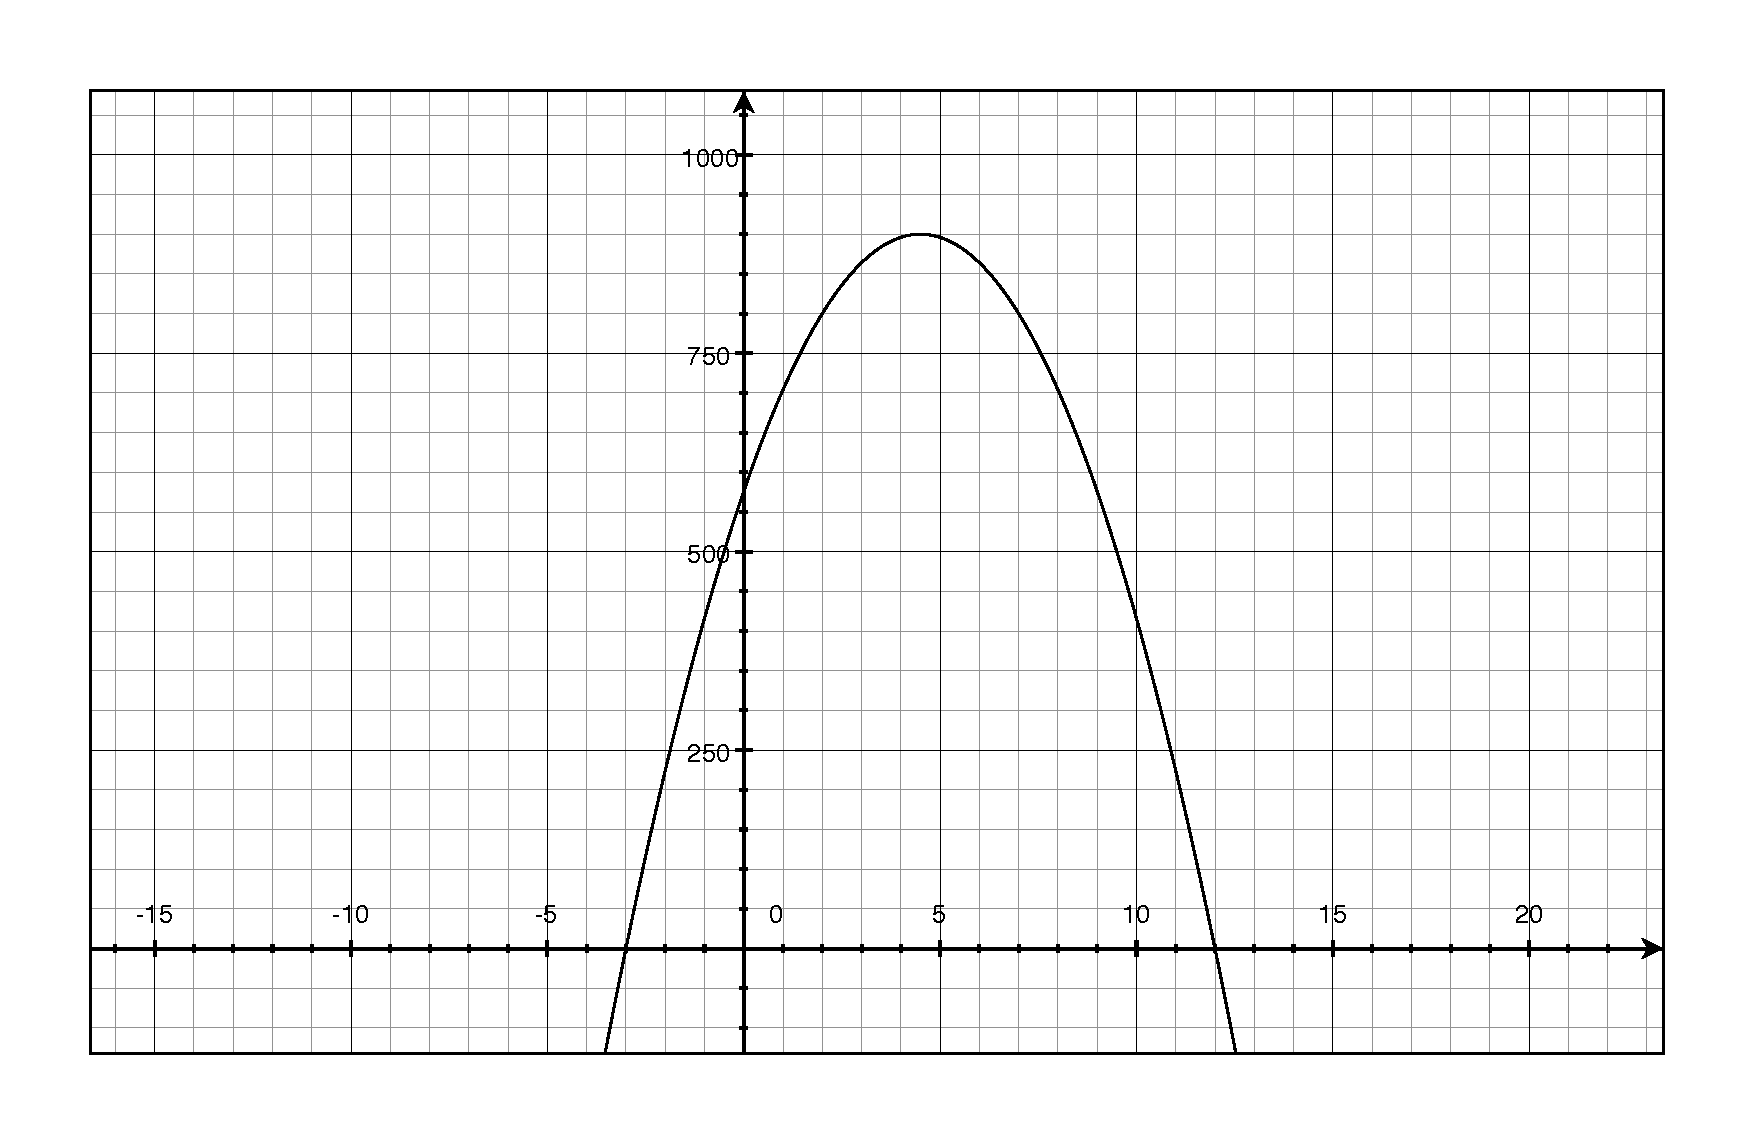
\includegraphics[width=7cm,height=5cm]{p65-25.eps}
  \caption*{Problem 25: $s(t) = 576 + 144t - 16t^2$}
\end{figure}

\item[b]
From part a, the rock hits the ground after 12 seconds.

\item[c]
From part a, the rock reaches its maximum height after 4.5 seconds

\item[d]
The rock is in the air from time 0 to time 12, so the domain is $[0, 12]$.  During this time, the rock will be between 0
and 900 feet, so the range is: $[0, 900]$.

\end{itemize}

\pagebreak

\item[26]
\begin{itemize}
\item[a]
$v(t) = -32t + 144$, so the graph is a line with slope $-32$ and y-intercept 144.

\begin{figure}[H]
  \centering
  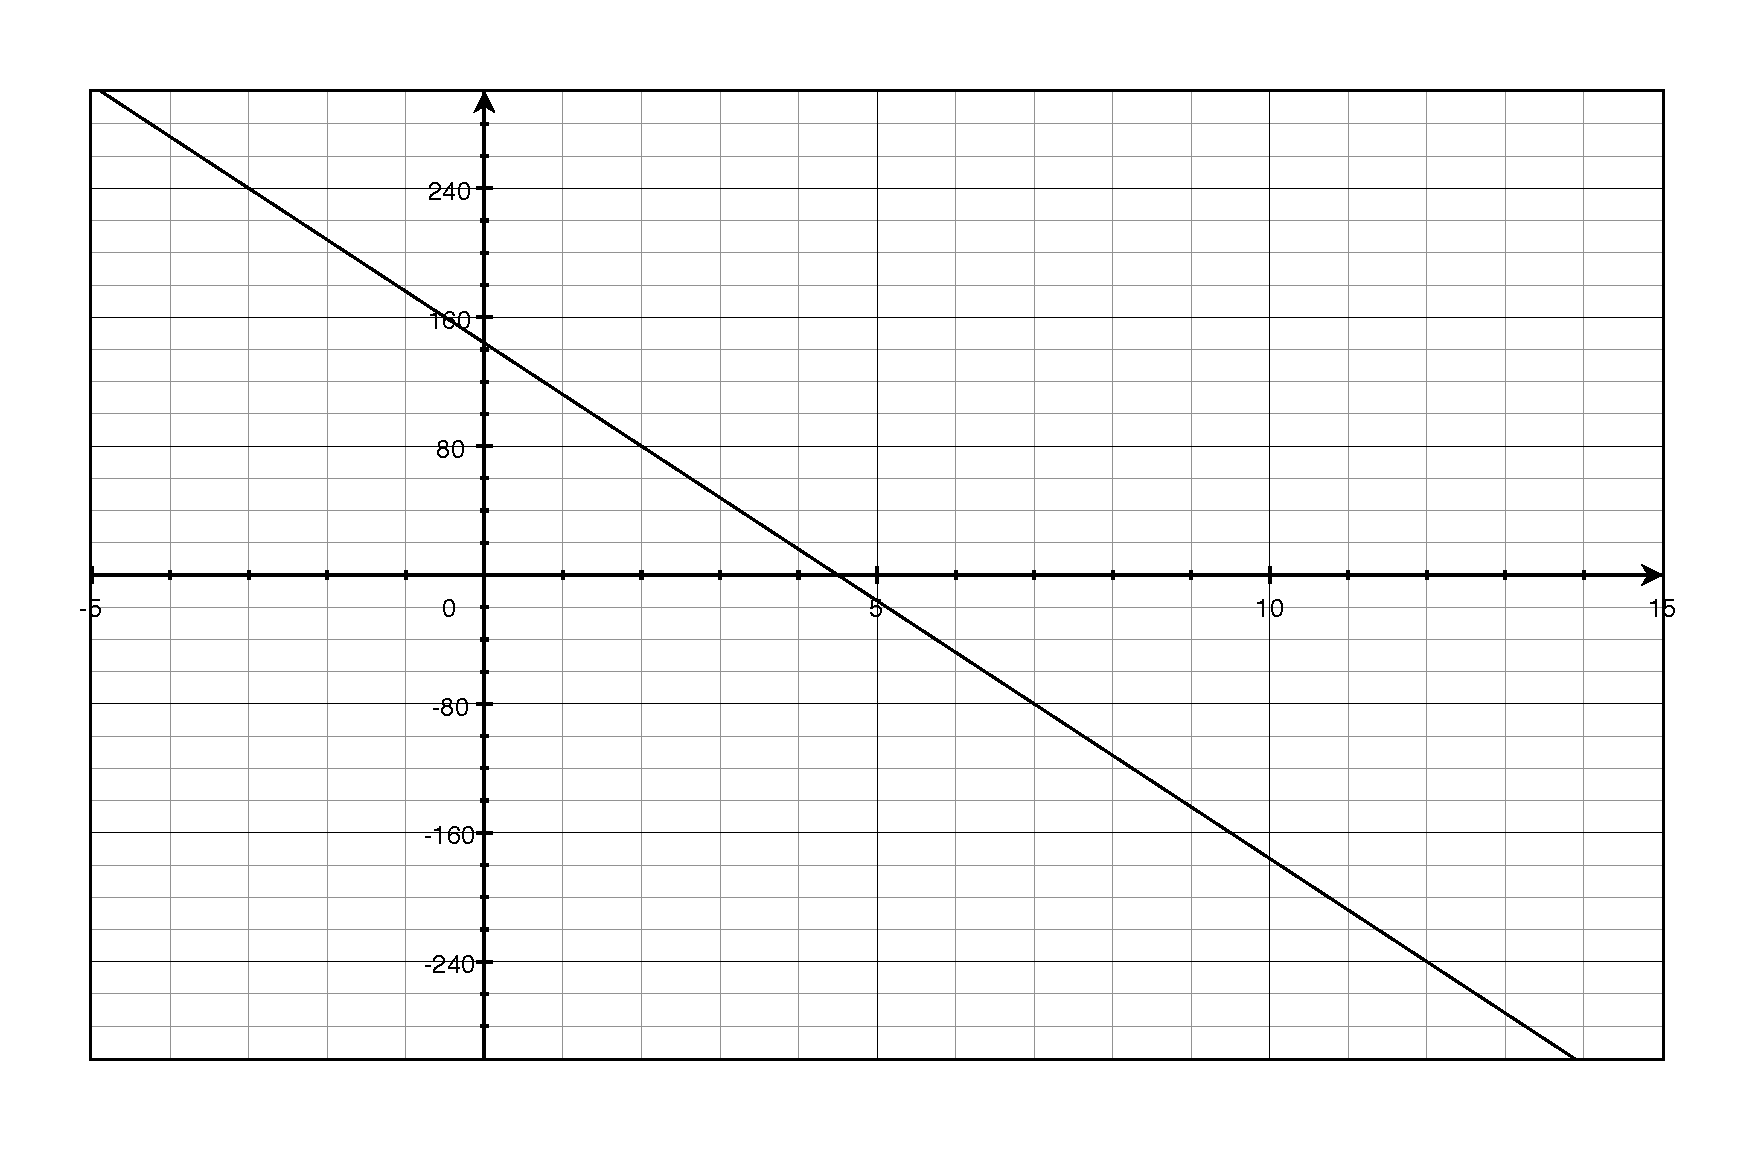
\includegraphics[width=7cm,height=5cm]{p65-26.eps}
  \caption*{Problem 26: $v(t) = -32t + 144$}
\end{figure}

\item[b]
From problem 26, the rock hits the ground after 12 seconds.  Its velocity at this time is:
\[
  v(12) = -32(12) + 144 = -240
\]

Notice that the velocity is positive until $t=4.5$.  This agrees with problem 25 which showed the rock reaching its
maximum height at 4.5 seconds.  After this point, the rock starts moving down, and its height starts to decrease.

If you look at the negative part of the graph, at time $-3$ the rock would have been traveling at +240 ft/sec if it
had been thrown from the ground instead of the top of the building.  So if you threw the rock straight up at time -3 at
+240 ft/sec, it would land on the ground at time 12 traveling at -240 ft/sec.

This brings up an interesting point regarding post-battle victory celebrations involving shooting guns in the air.  If
you shoot your gun in the air, the bullet will eventually land on your head at about the same velocity as it originally
left the gun.  So if you do shoot straight up into the air in a celebratory way, you should make sure you move before
the bullet lands.

\item[c]
The domain is the same is problem 25, or $[0, 12]$.  The rock is going fastest when it is first thrown upwards at 
144 ft/s.  It hits the ground going $-240$ ft/s, so the range is: $[-240, 144]$.

\end{itemize}

\item[27]
Since this is the equation of a parabola, the minimum cost occurs at the vertex.  To find the vertex:

\[
  x_{vertex} = \frac{- (-120)}{2} = 60
\]

\[
  C(60) = 60^2 - 120(60) + 4000 = 400
\]

So producing 60 units per day will result in the minimum cost of \$400/unit.

\item[28]
Since this is the equation of an inverted parabola, the maximum cost occurs at the vertex.  To find the vertex:

\[
  x_{vertex} = \frac{-160)}{2(-0.1)} = 800
\]

\[
  P(60) = -0.1(800)^2 + 160(800) - 20,000 = 44,000
\]

So selling 800 terminals/month will result in the maximum profit of \$44,000.

\end{itemize}

\section{Page 73}
\begin{itemize}

\item[3]
\begin{figure}[H]
  \centering
  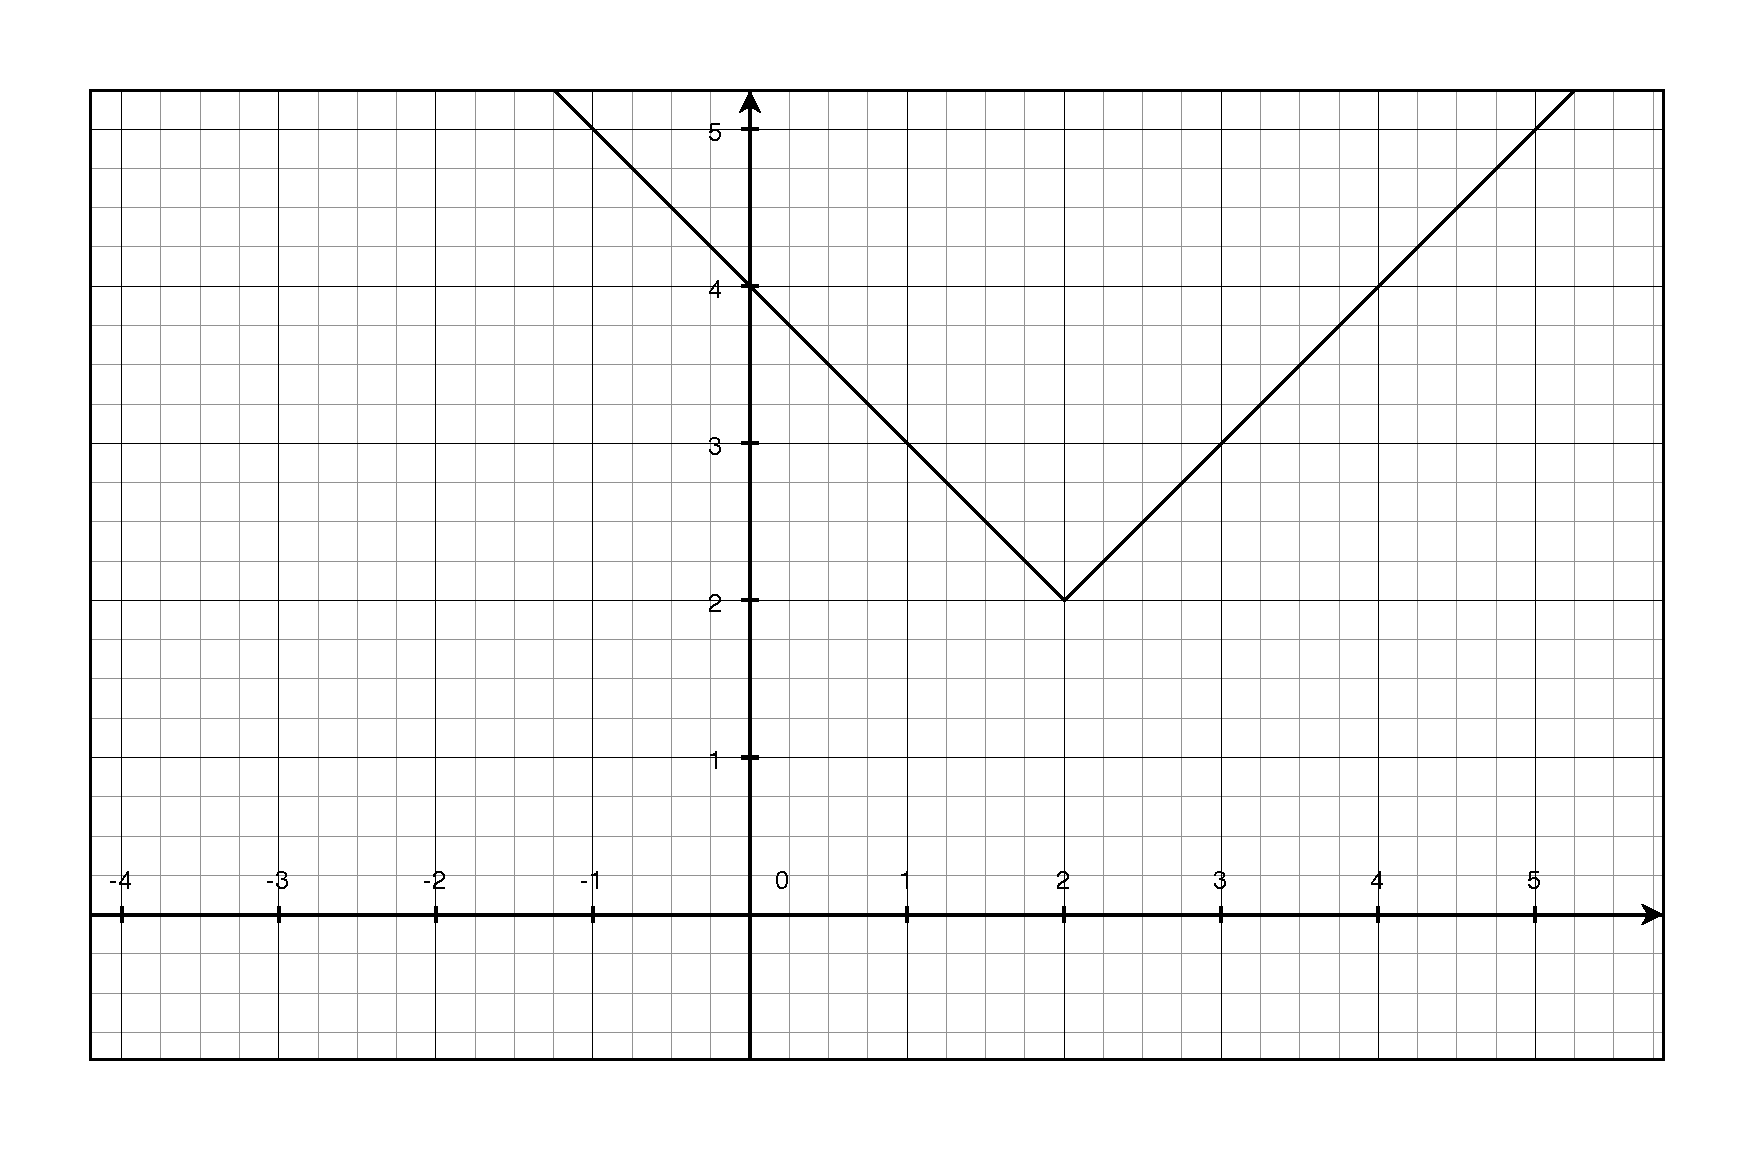
\includegraphics[width=7cm,height=5cm]{1.9-3.eps}
  \caption*{Problem 3}
\end{figure}

\item[6]

\begin{align*}
  f(x) &= |2x-5| \\
  &= \left| 2 \left( x-\frac{5}{2} \right) \right| \\
  &= 2 \left| x-\frac{5}{2} \right| \\
\end{align*}

\begin{figure}[H]
  \centering
  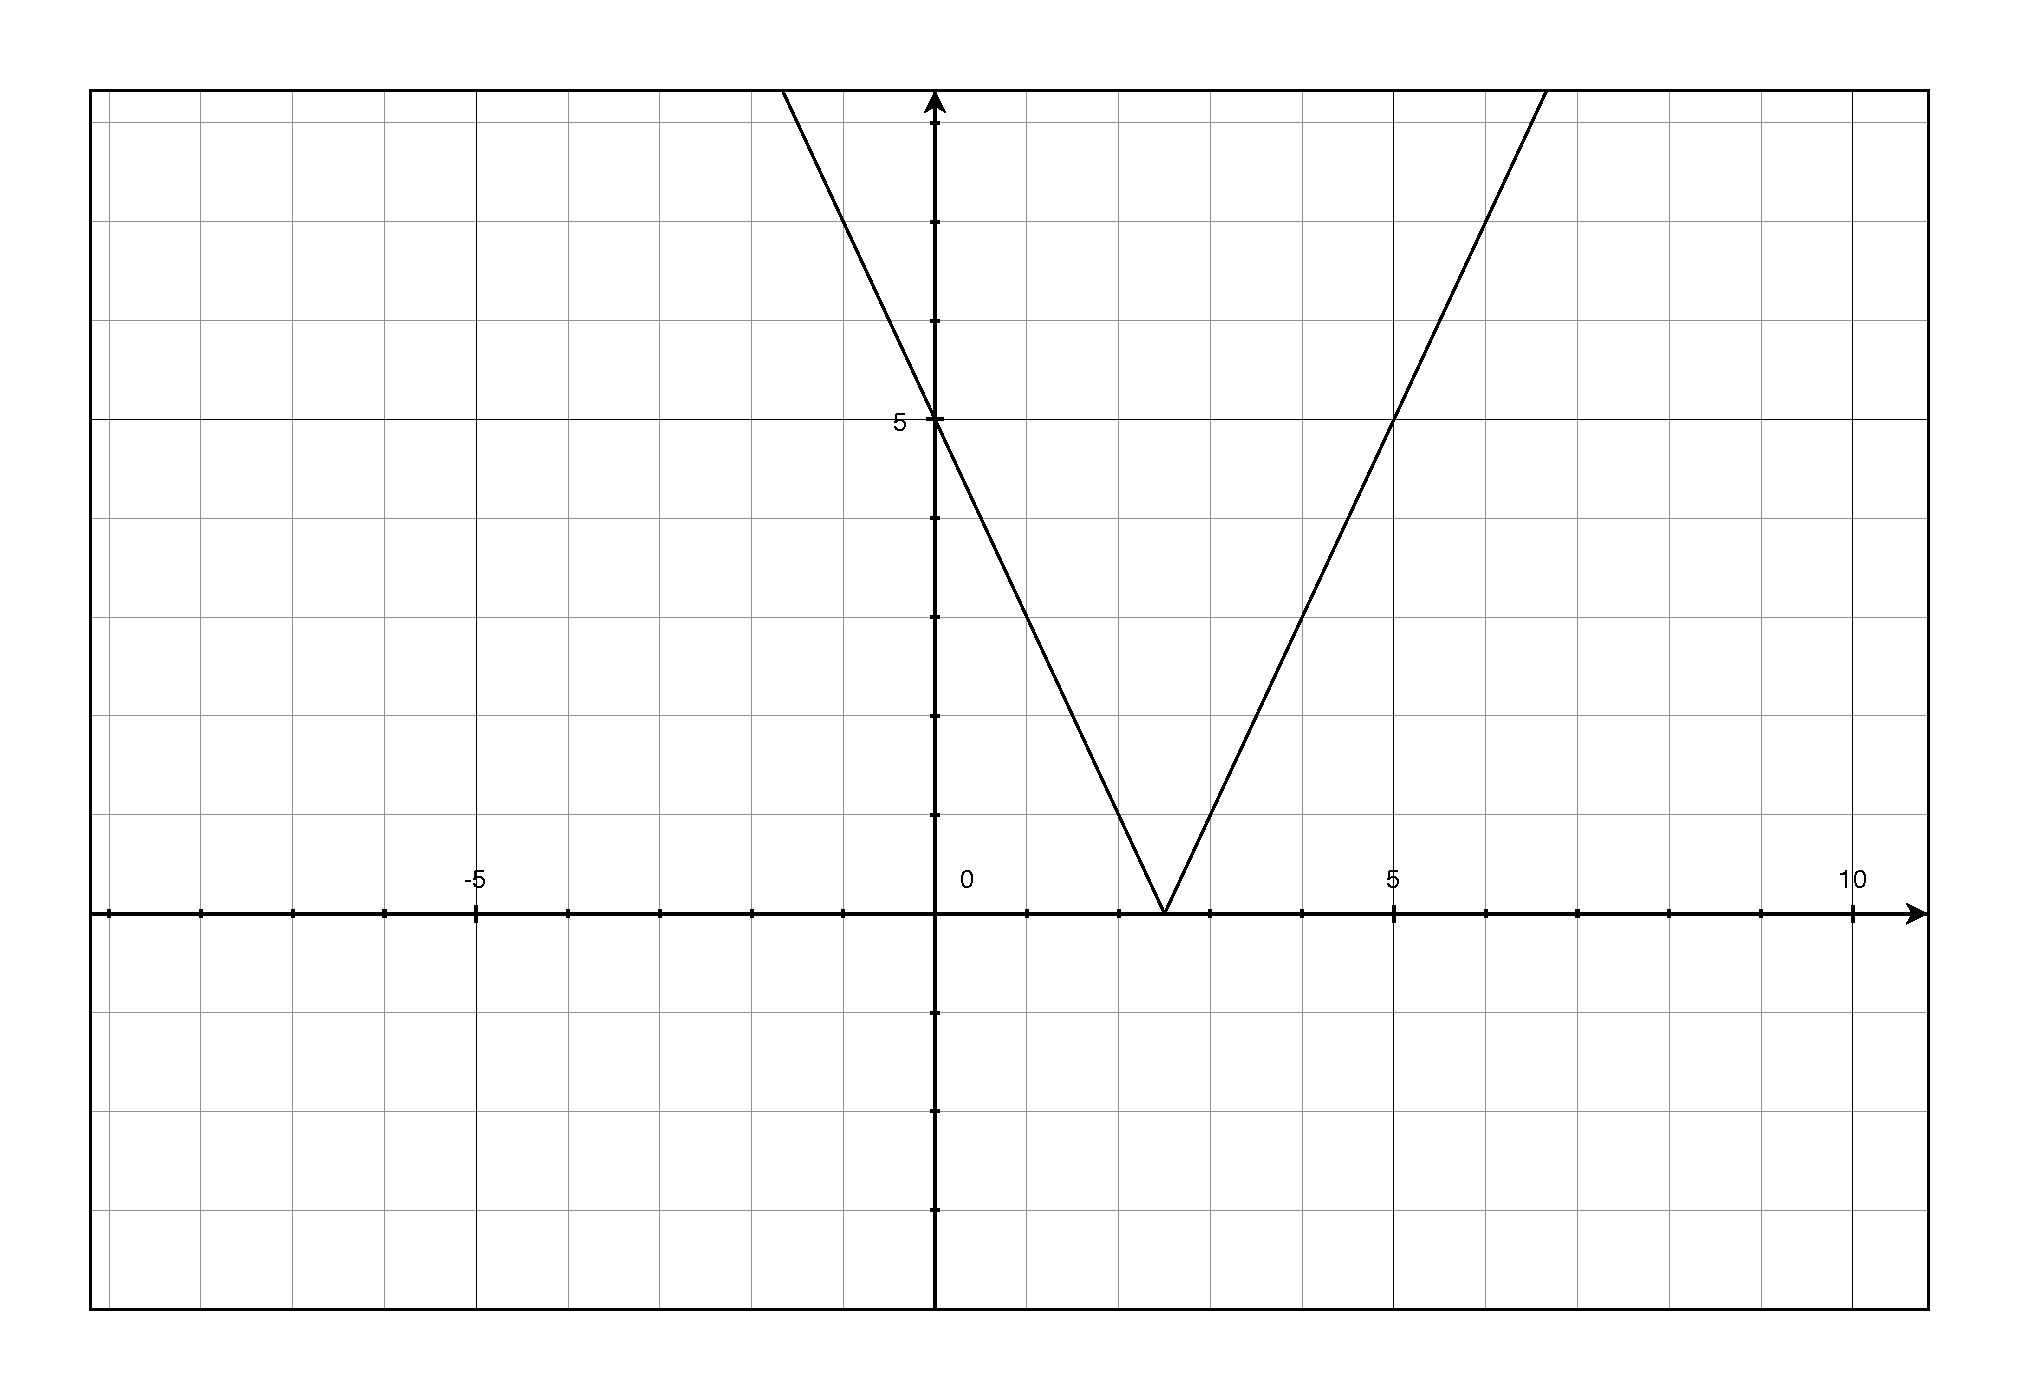
\includegraphics[width=7cm,height=5cm]{1.9-6.eps}
  \caption*{Problem 6: $f(x) = |2x-5|$}
\end{figure}

\item[8]
\begin{figure}[H]
  \centering
  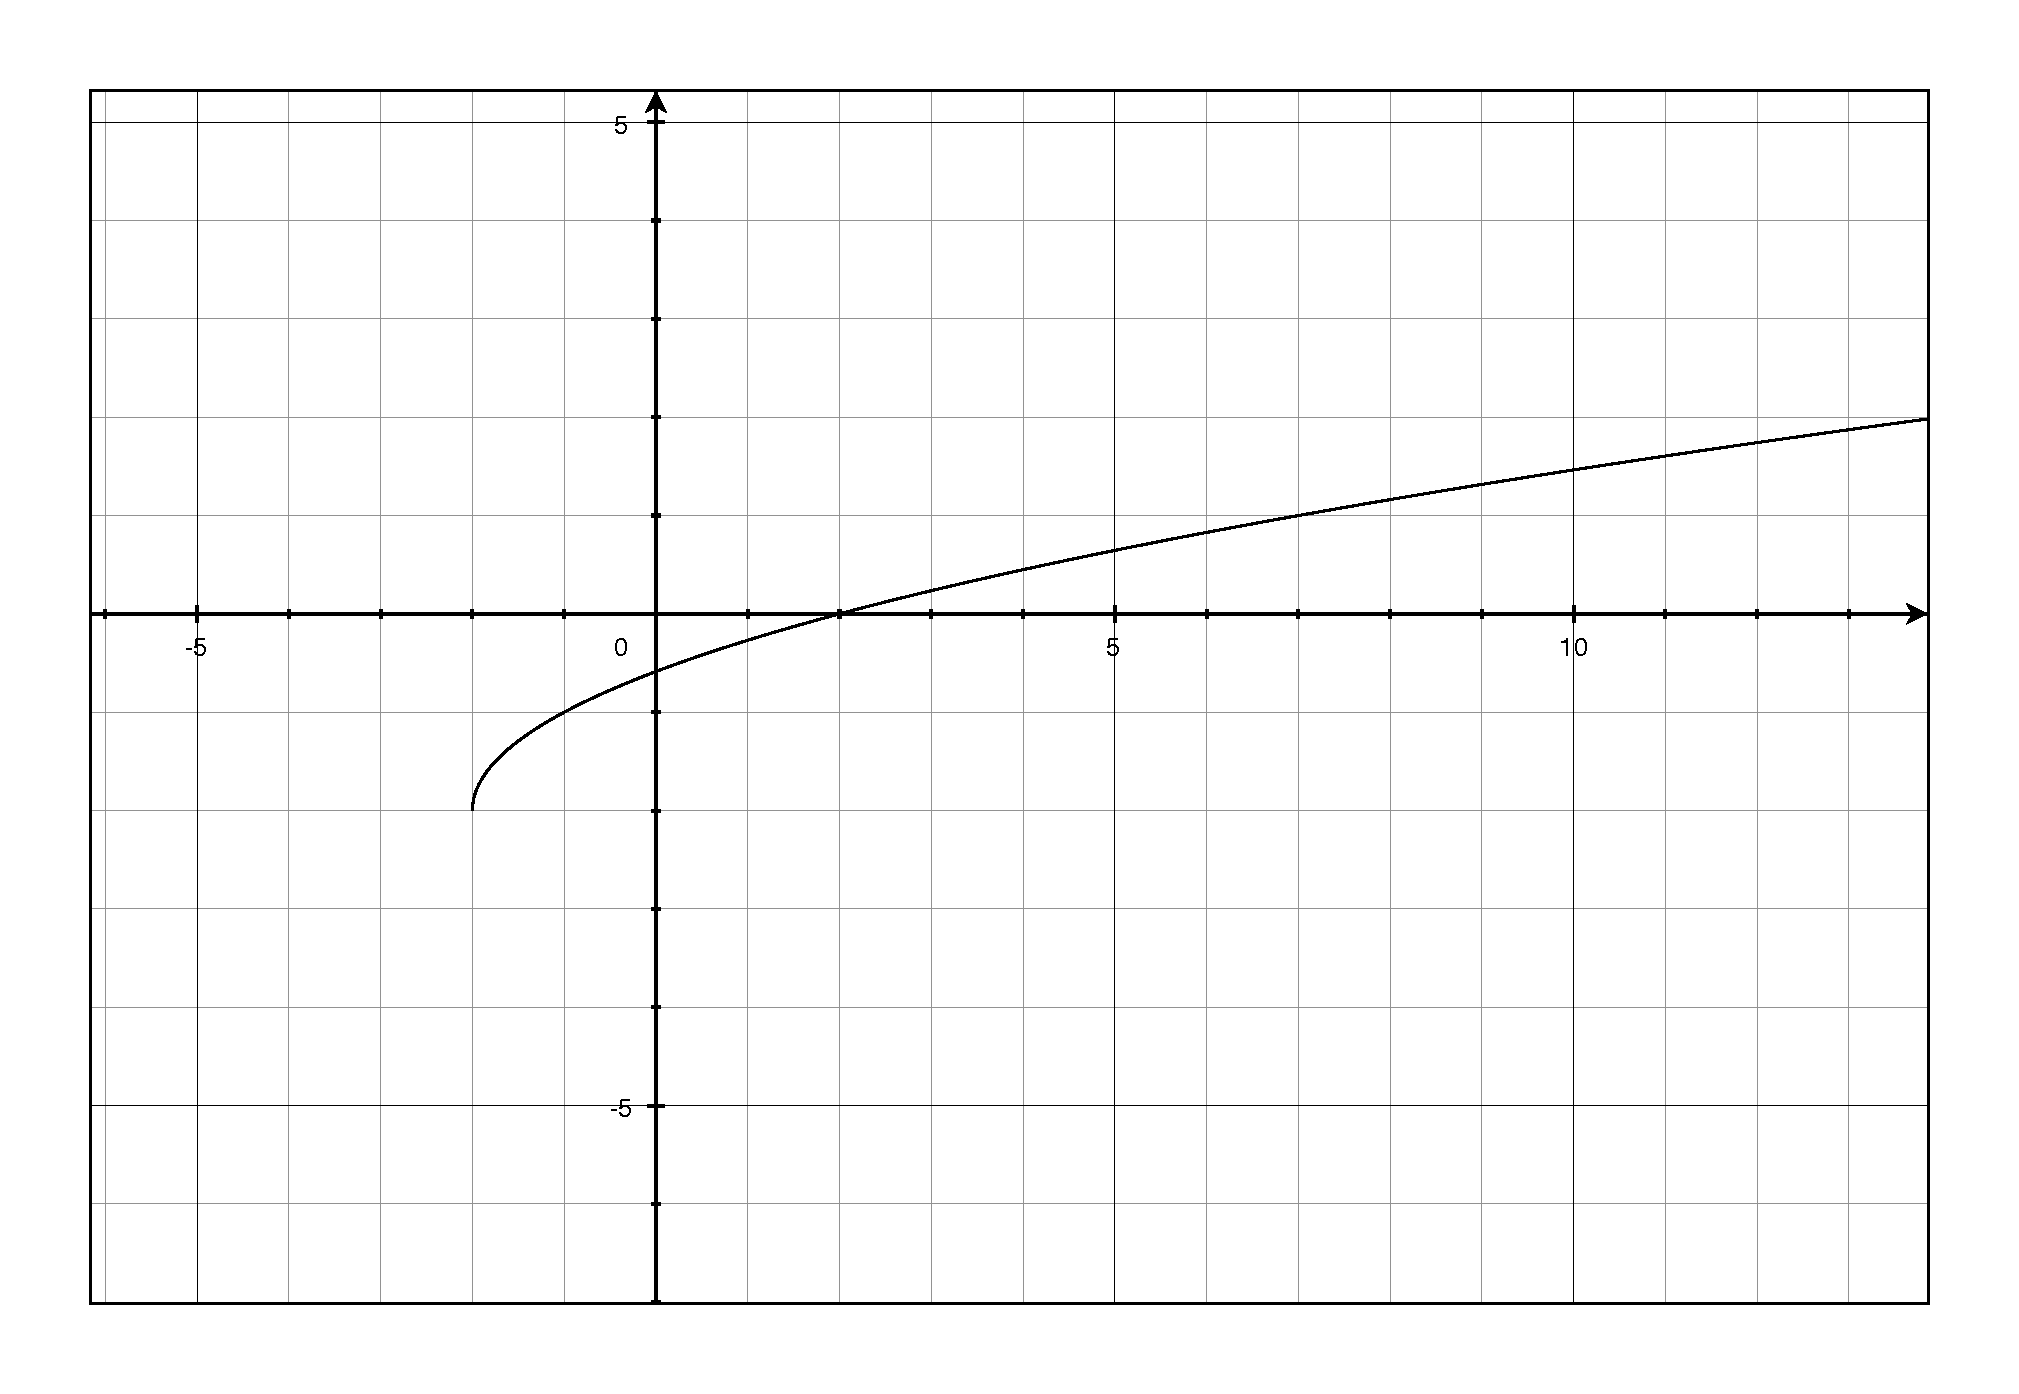
\includegraphics[width=7cm,height=5cm]{1.9-8.eps}
  \caption*{Problem 8: $f(x) = |2x-5|$}
\end{figure}

\item[12]

\begin{figure}[H]
  \centering
  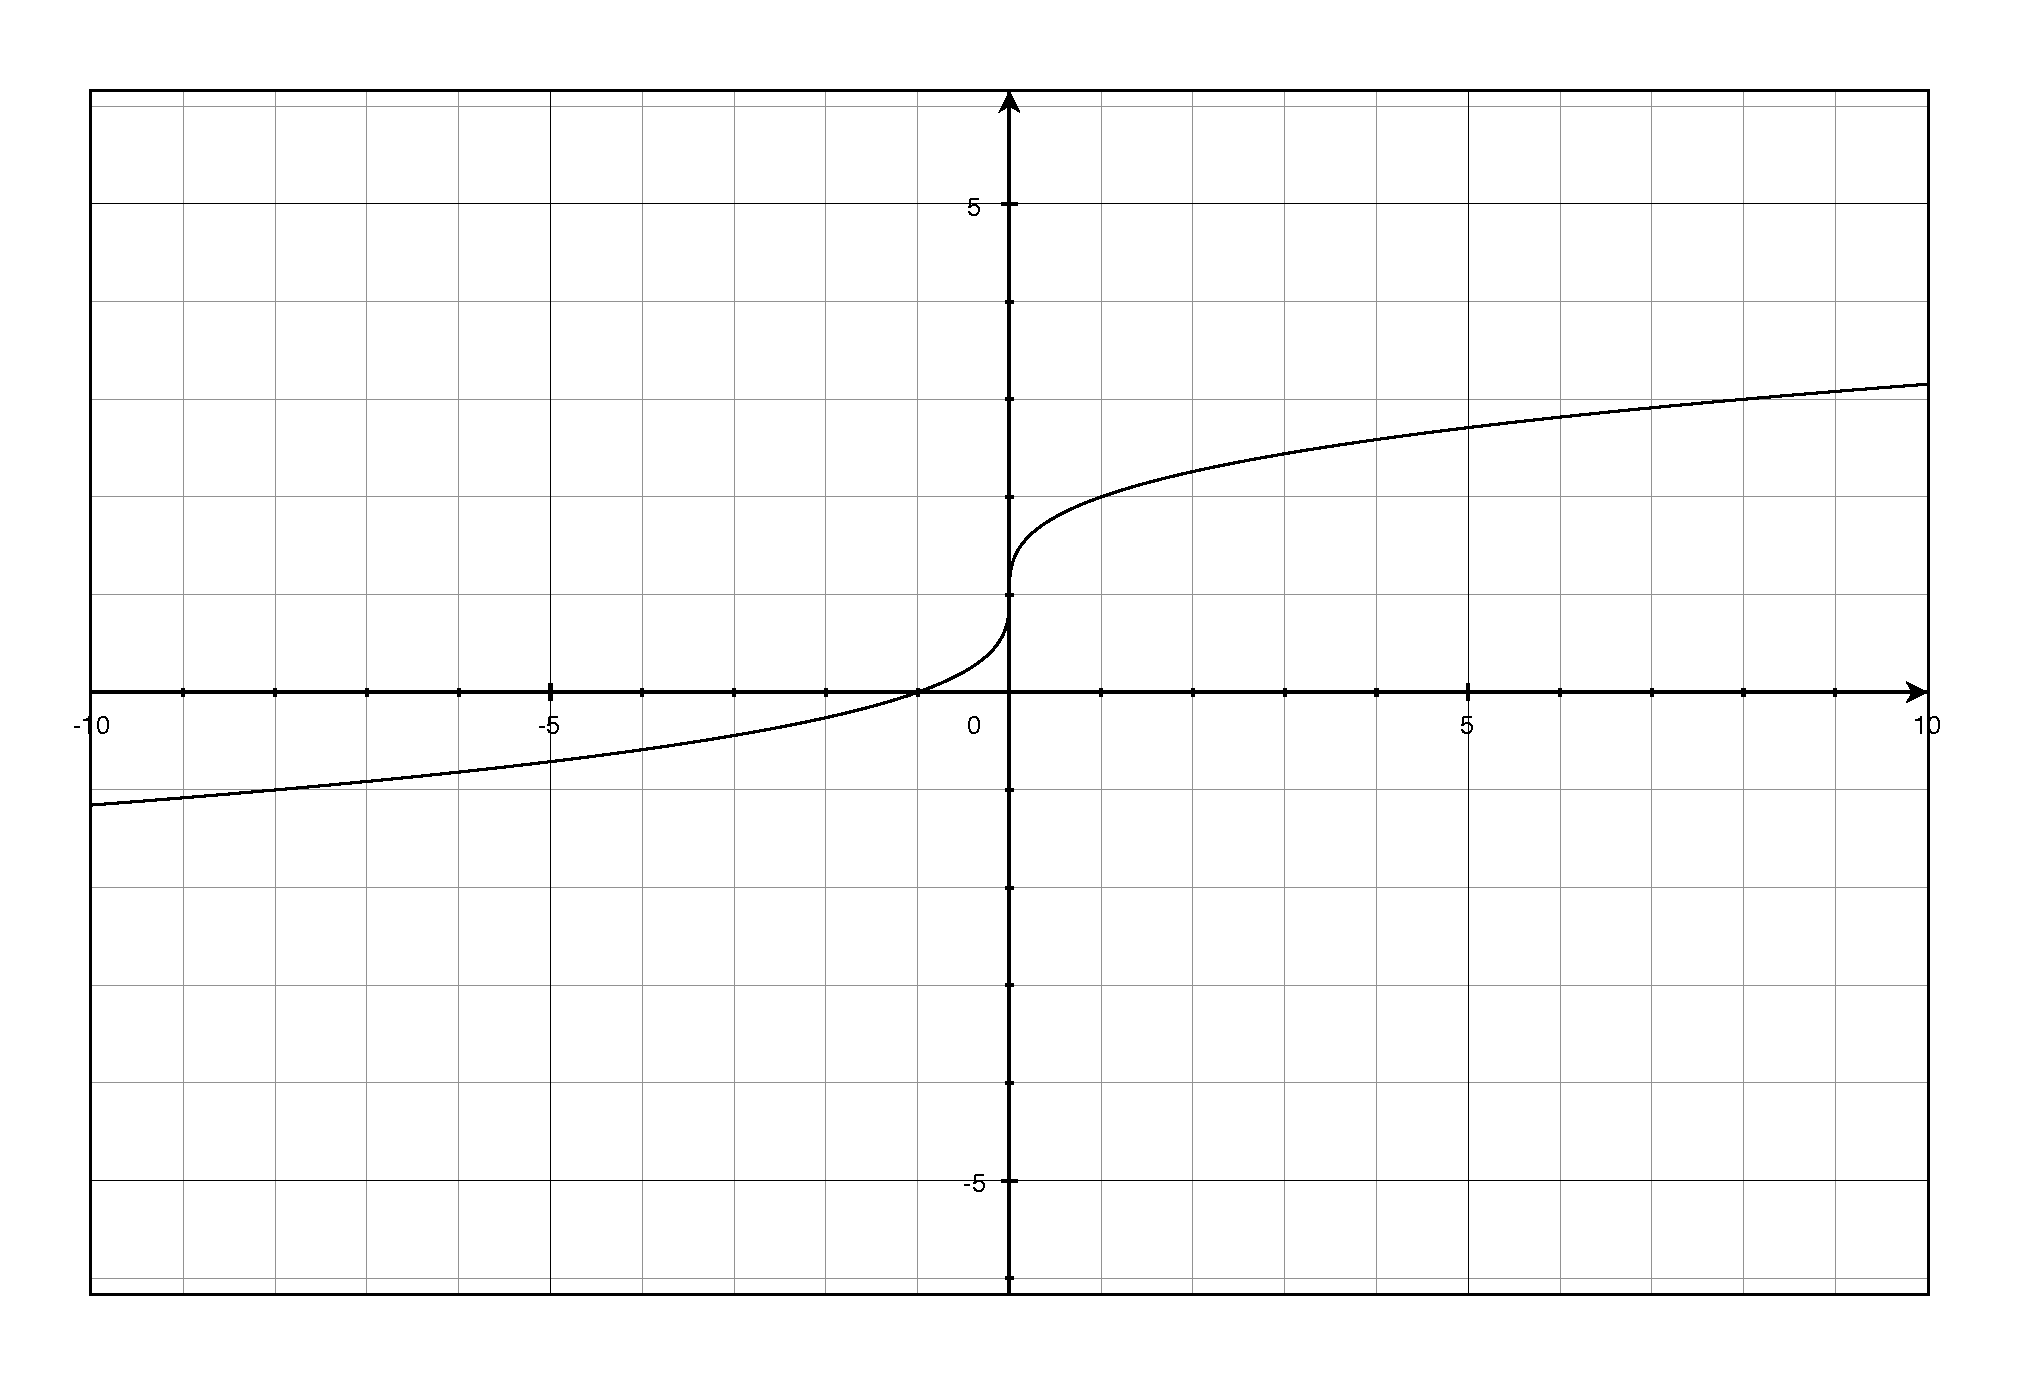
\includegraphics[width=7cm,height=5cm]{1.9-12a.eps}
  \caption*{Problem 12a: $g(x) = \sqrt[3]{x} + 1$}
\end{figure}

\begin{figure}[H]
  \centering
  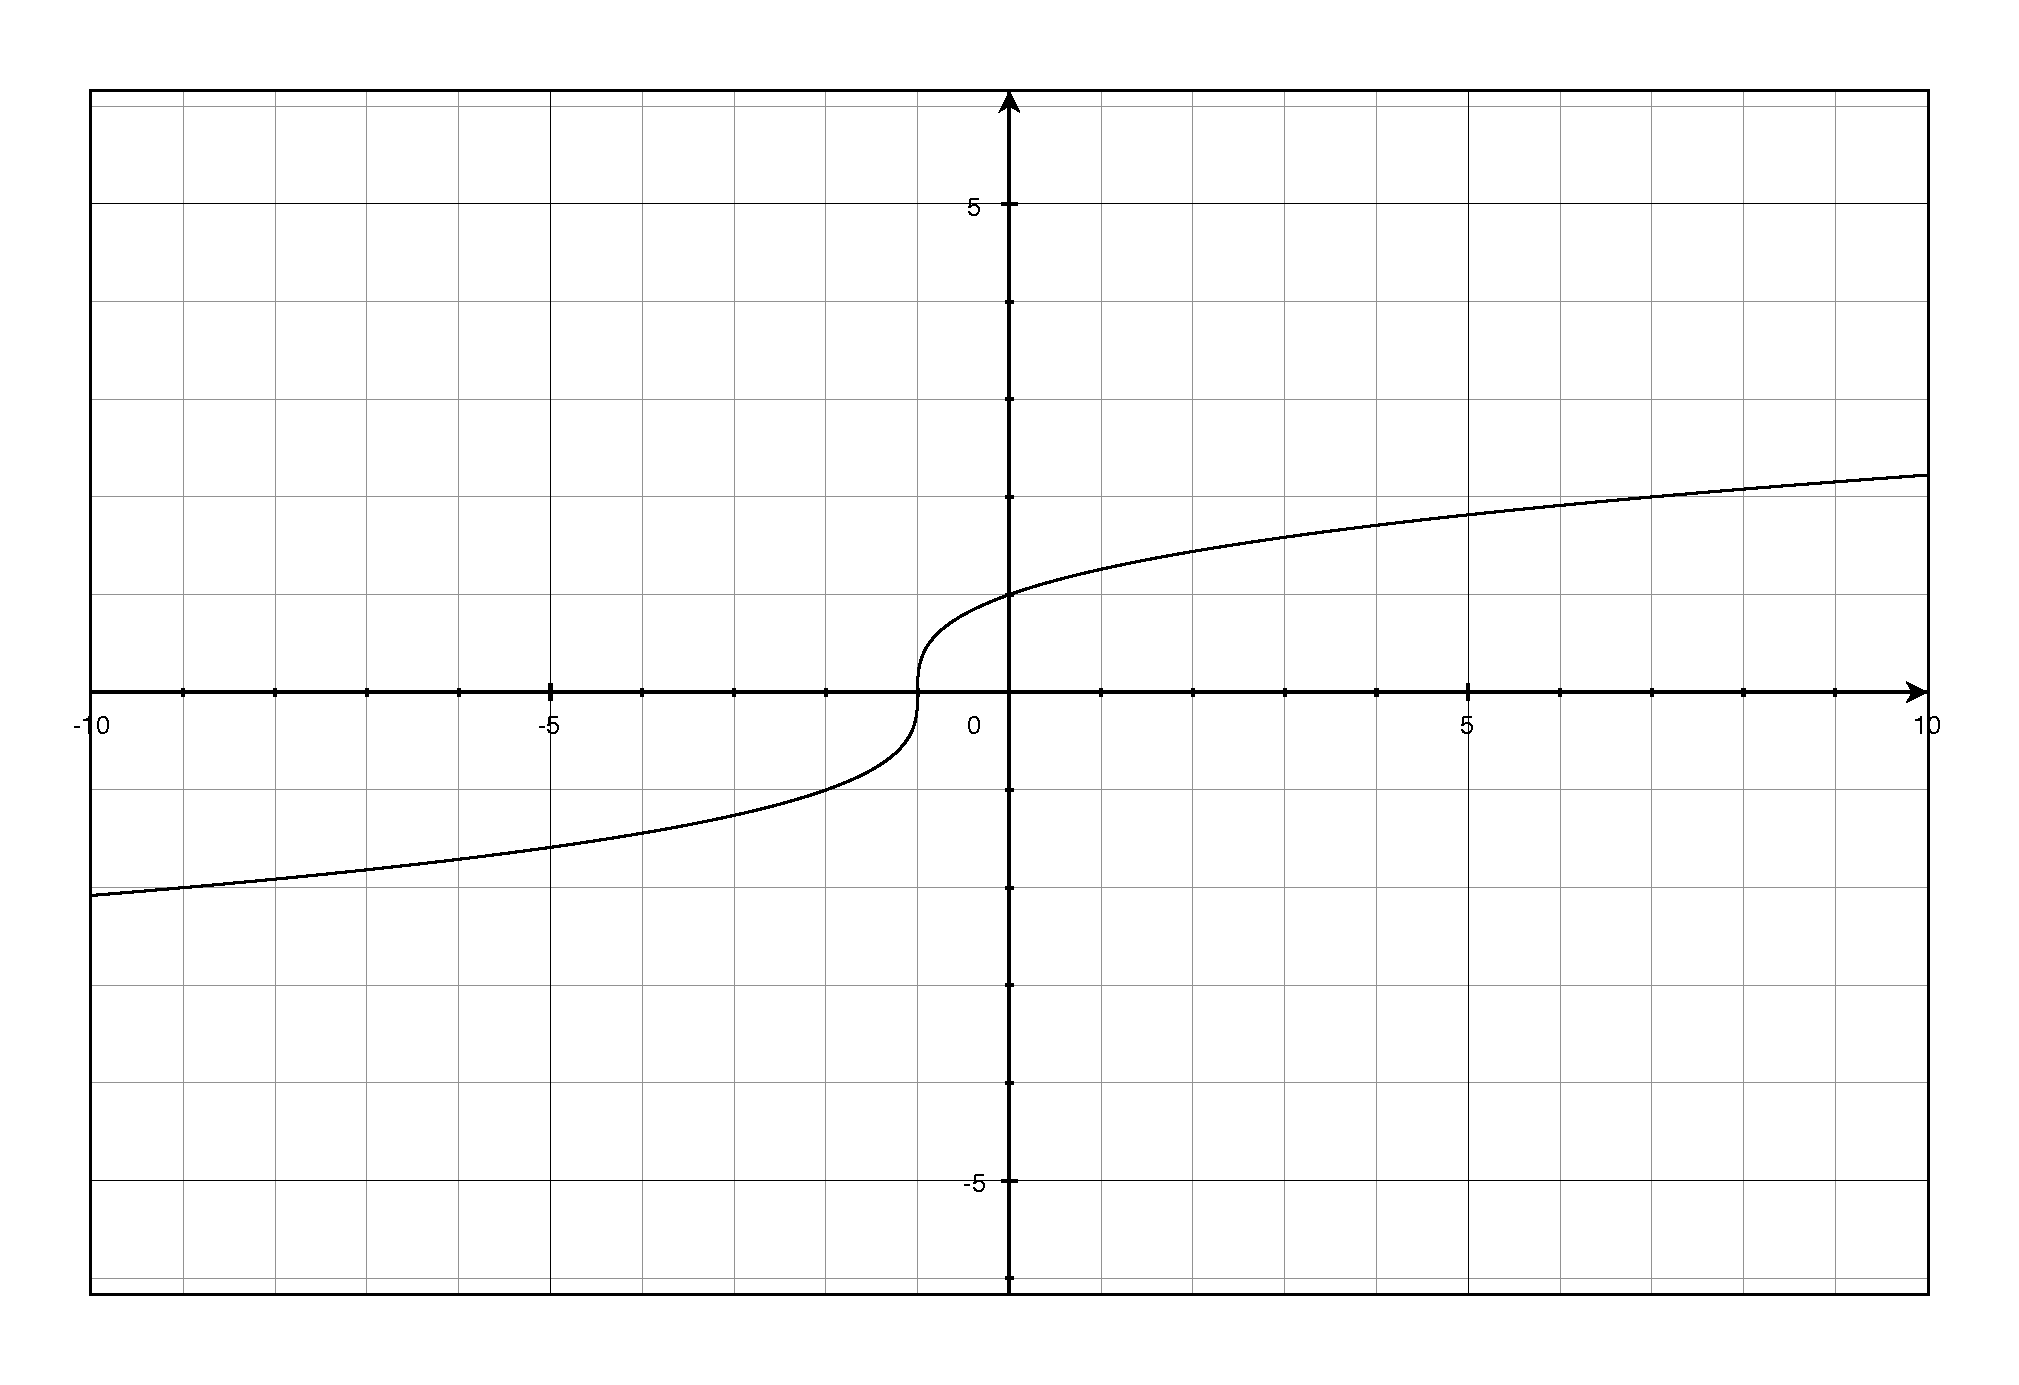
\includegraphics[width=7cm,height=5cm]{1.9-12b.eps}
  \caption*{Problem 12b: $g(x) = \sqrt[3]{x + 1}$}
\end{figure}

\begin{figure}[H]
  \centering
  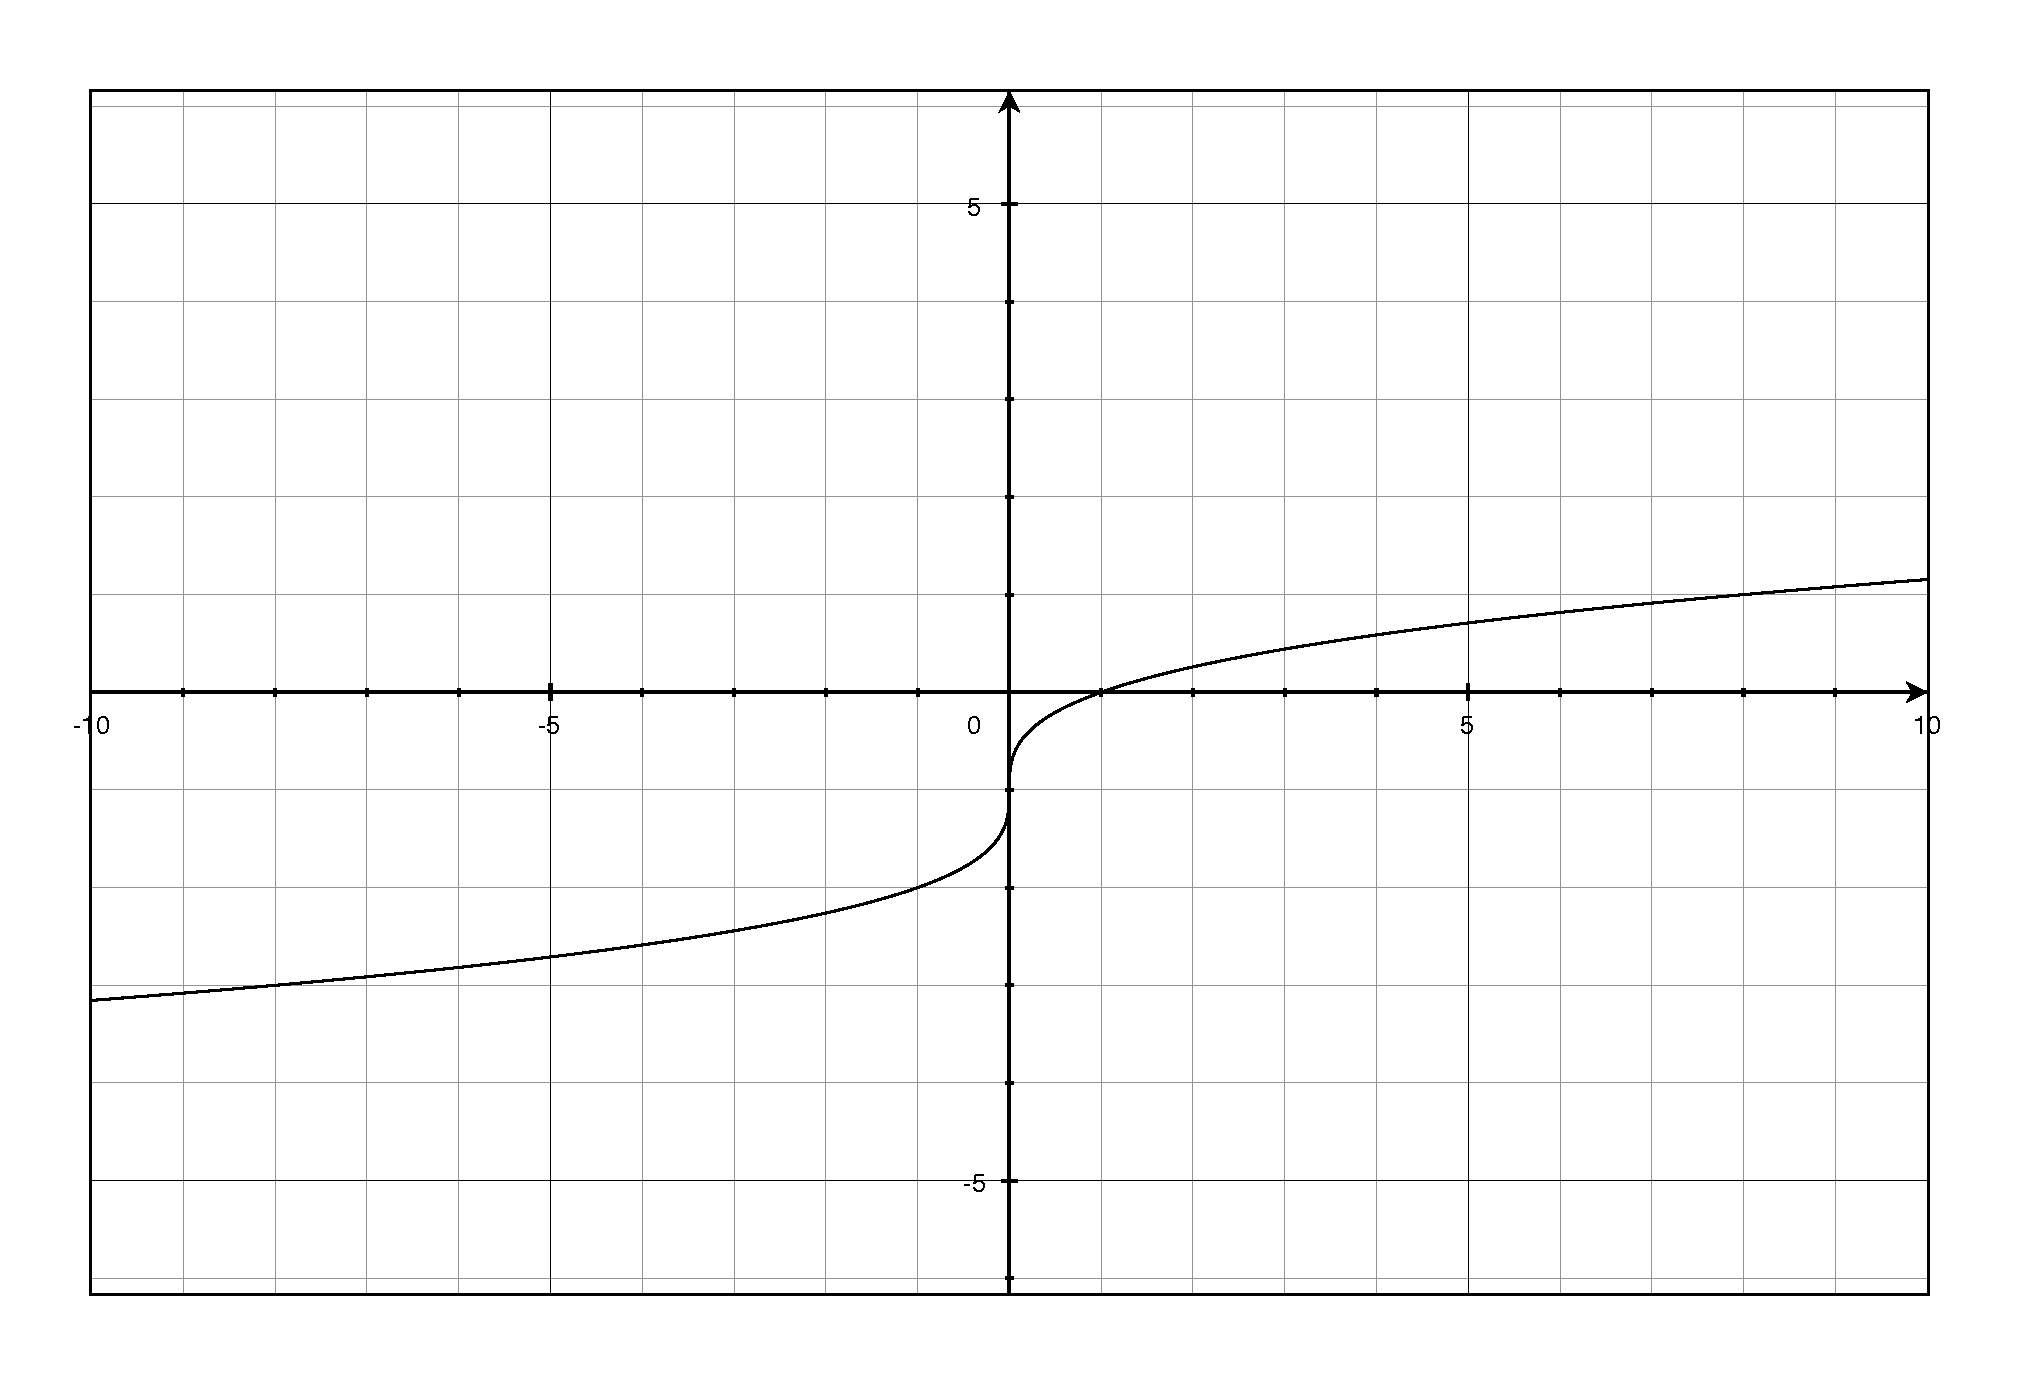
\includegraphics[width=7cm,height=5cm]{1.9-12c.eps}
  \caption*{Problem 12c: $g(x) = \sqrt[3]{x} - 1$}
\end{figure}

\begin{figure}[H]
  \centering
  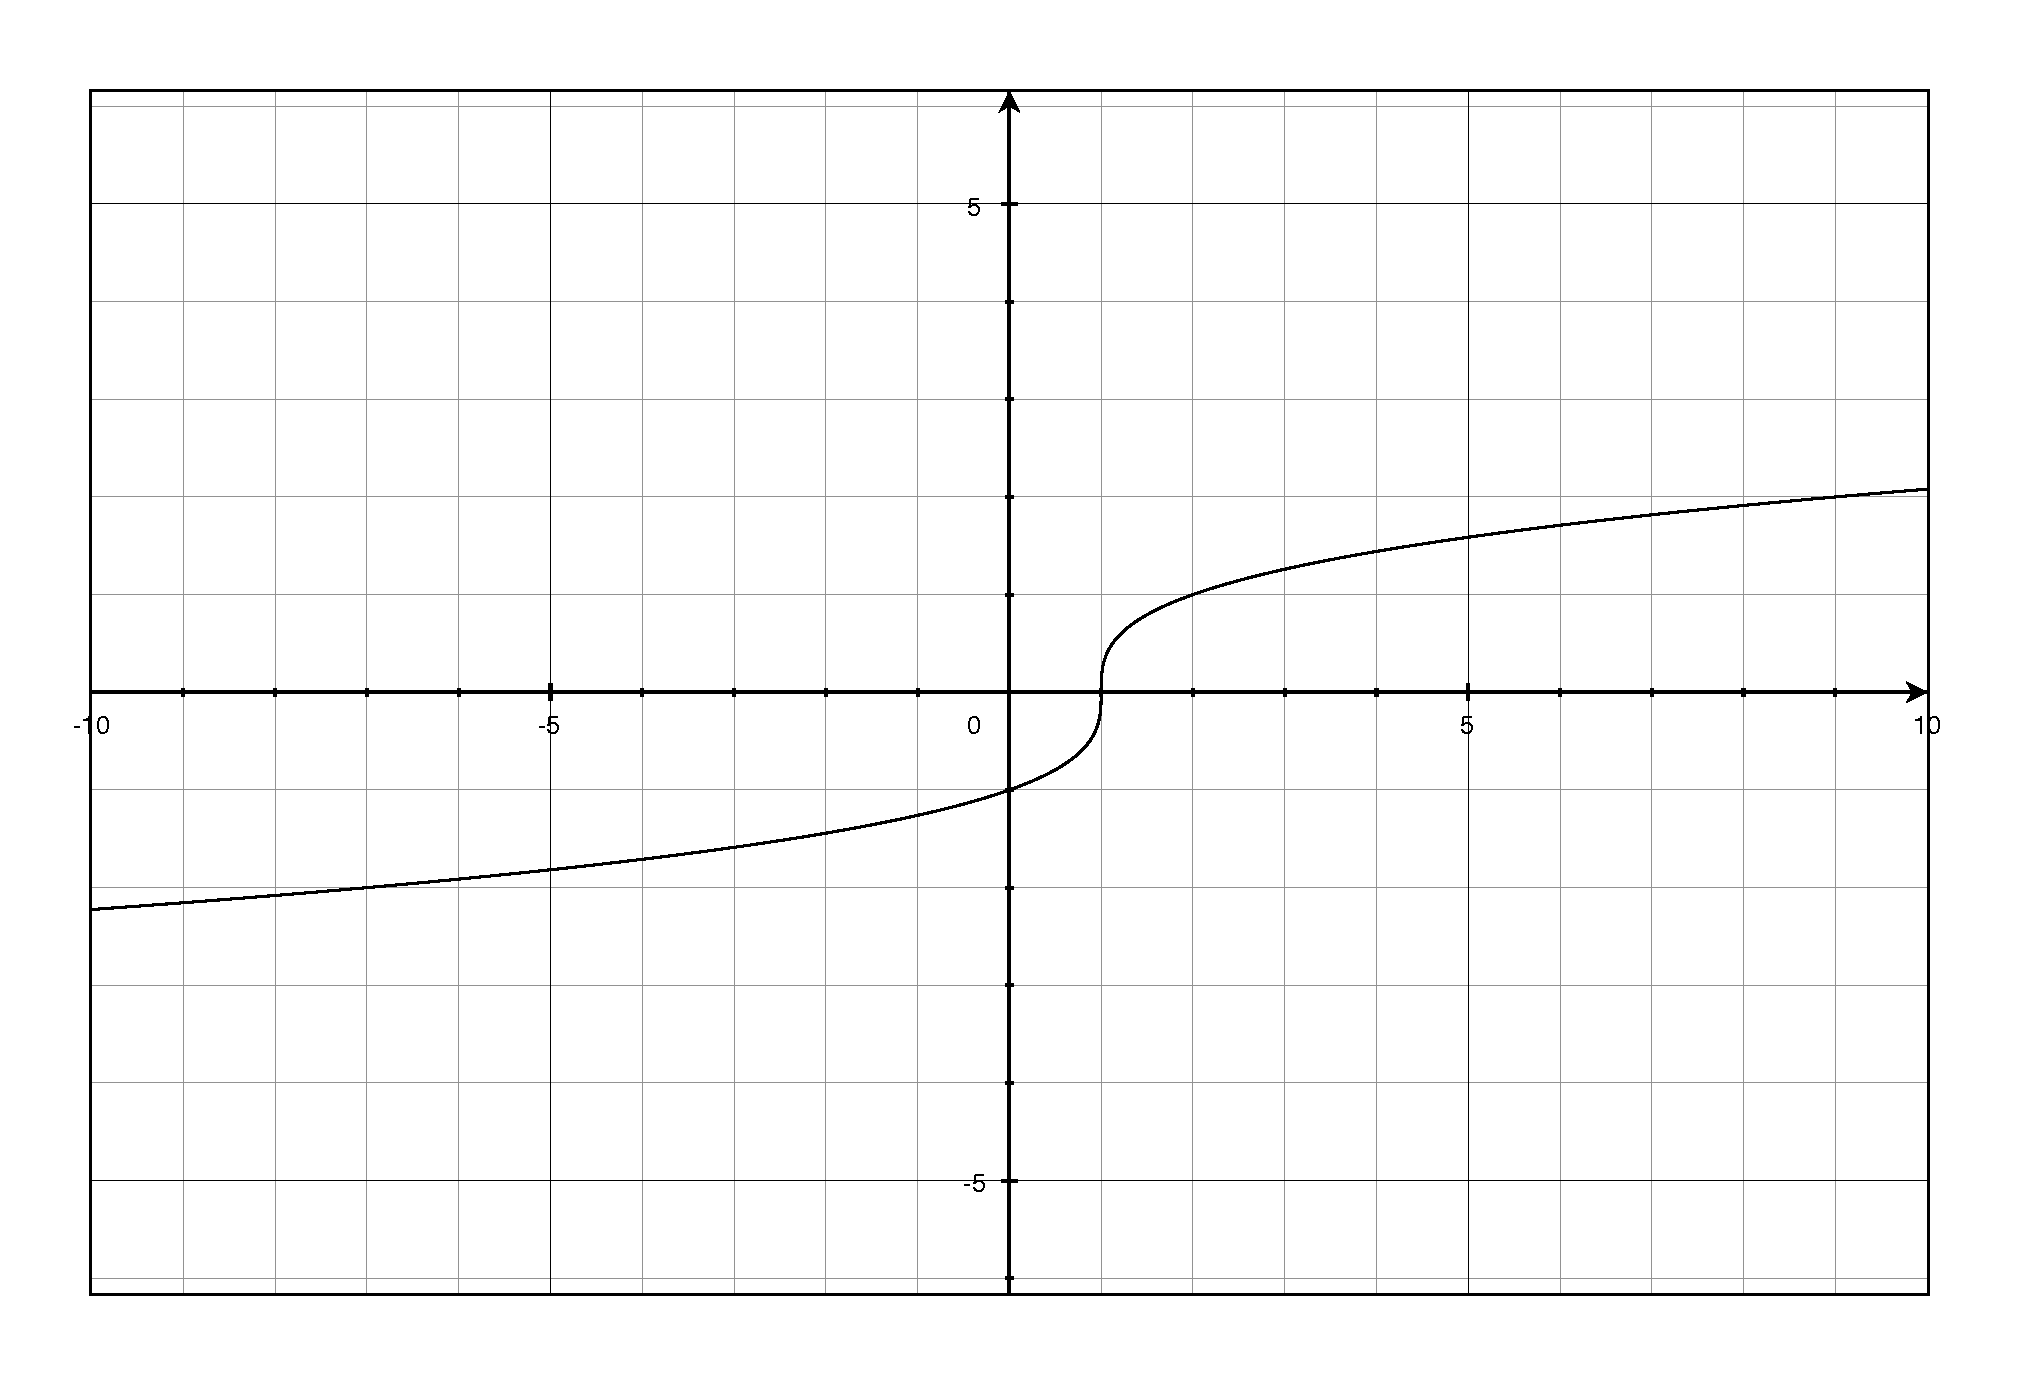
\includegraphics[width=7cm,height=5cm]{1.9-12d.eps}
  \caption*{Problem 12d: $g(x) = \sqrt[3]{x - 1}$}
\end{figure}

\begin{figure}[H]
  \centering
  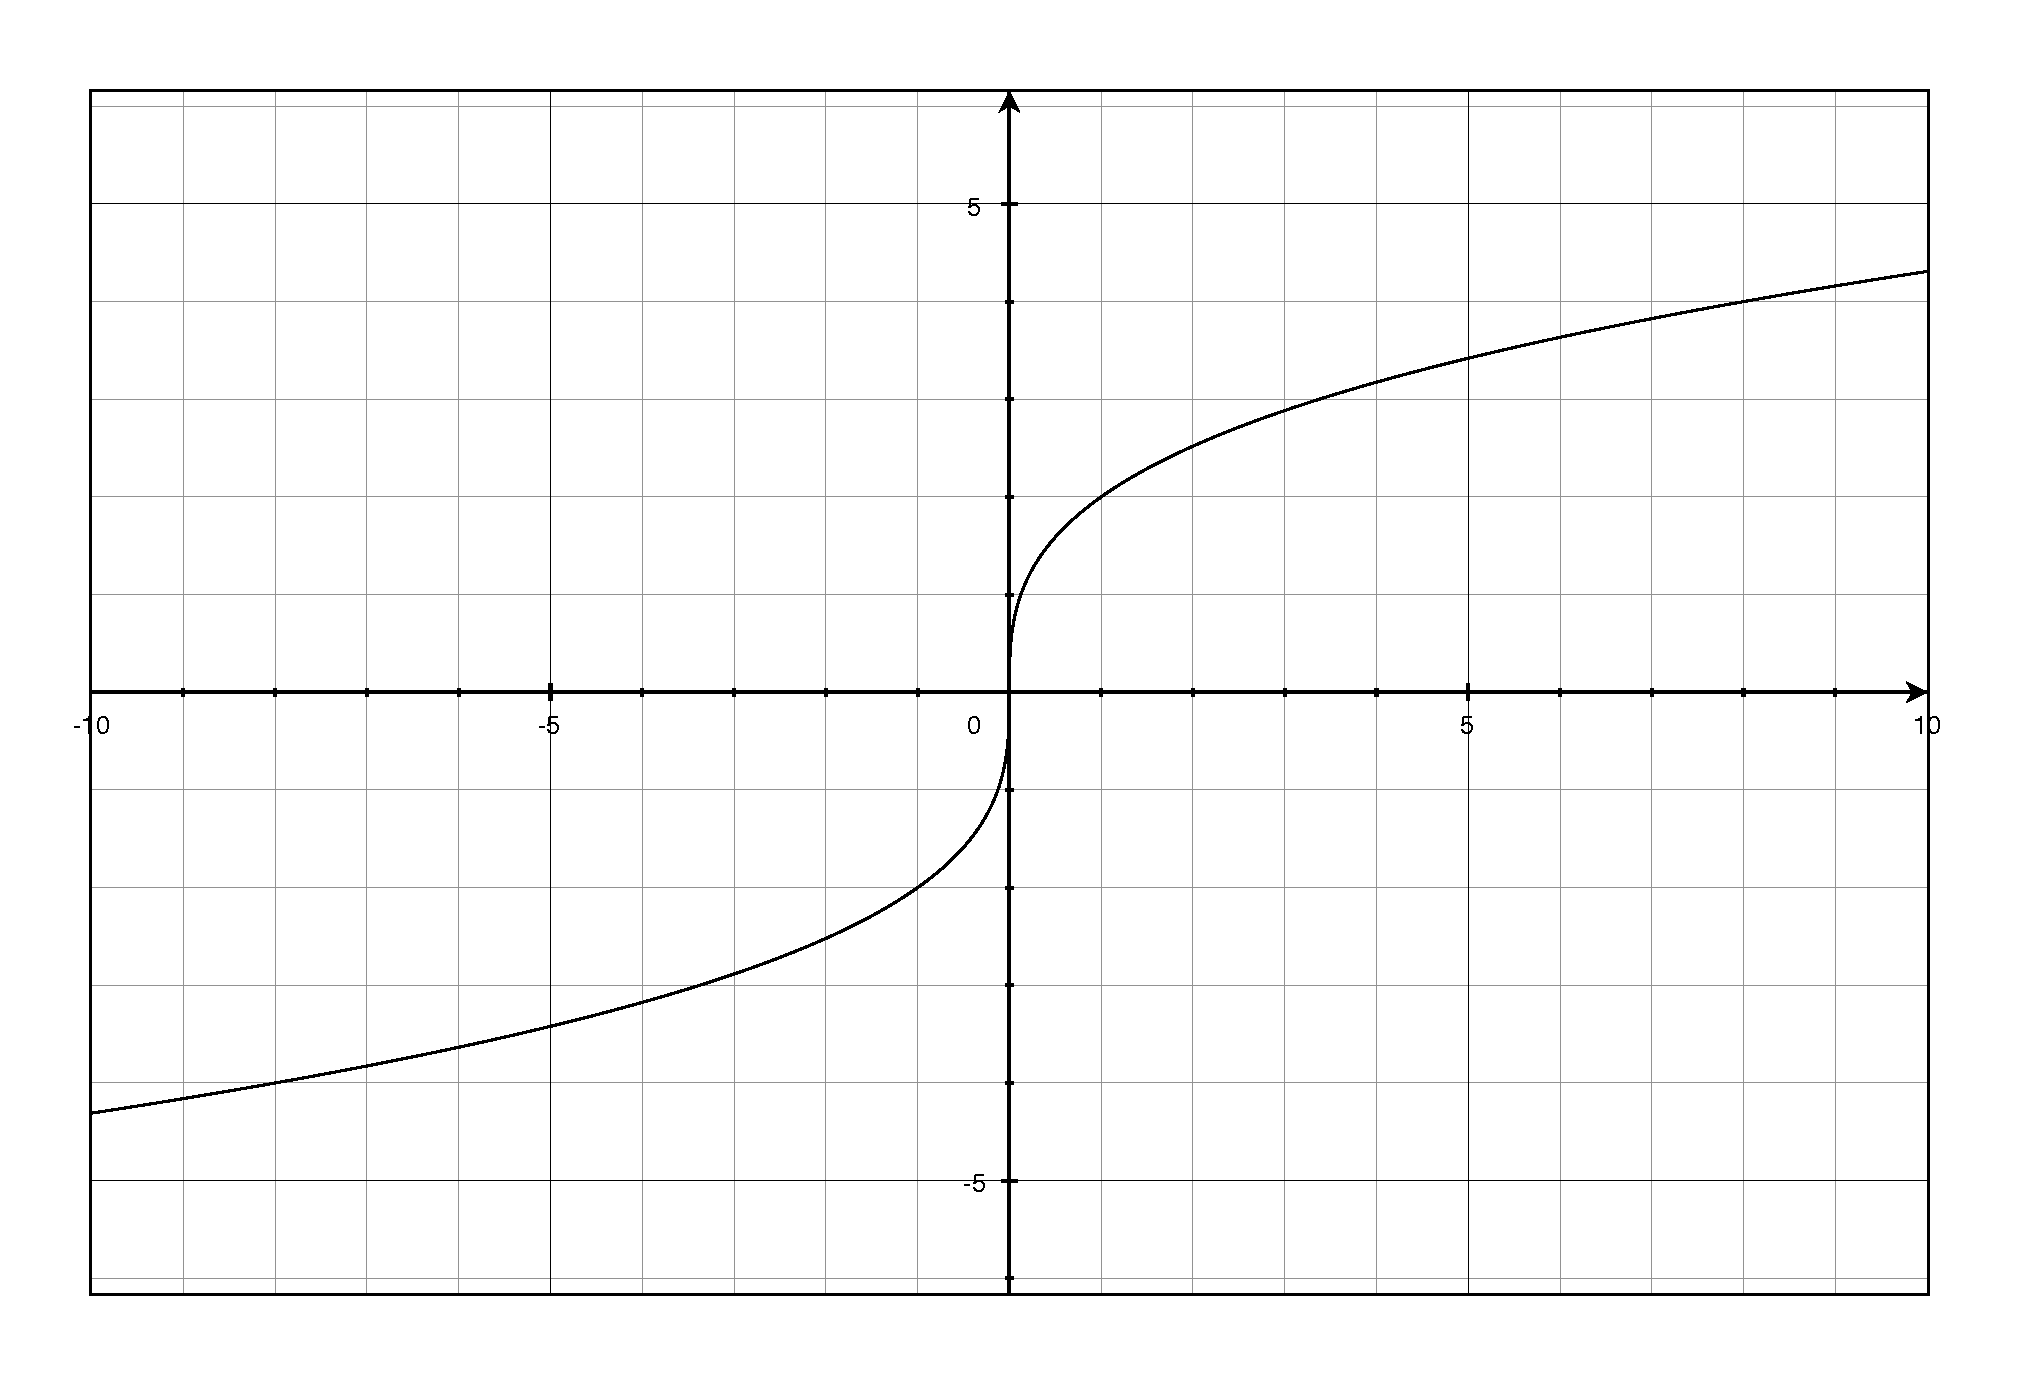
\includegraphics[width=7cm,height=5cm]{1.9-12e.eps}
  \caption*{Problem 12e: $g(x) = 2\sqrt[3]{x}$}
\end{figure}

\begin{figure}[H]
  \centering
  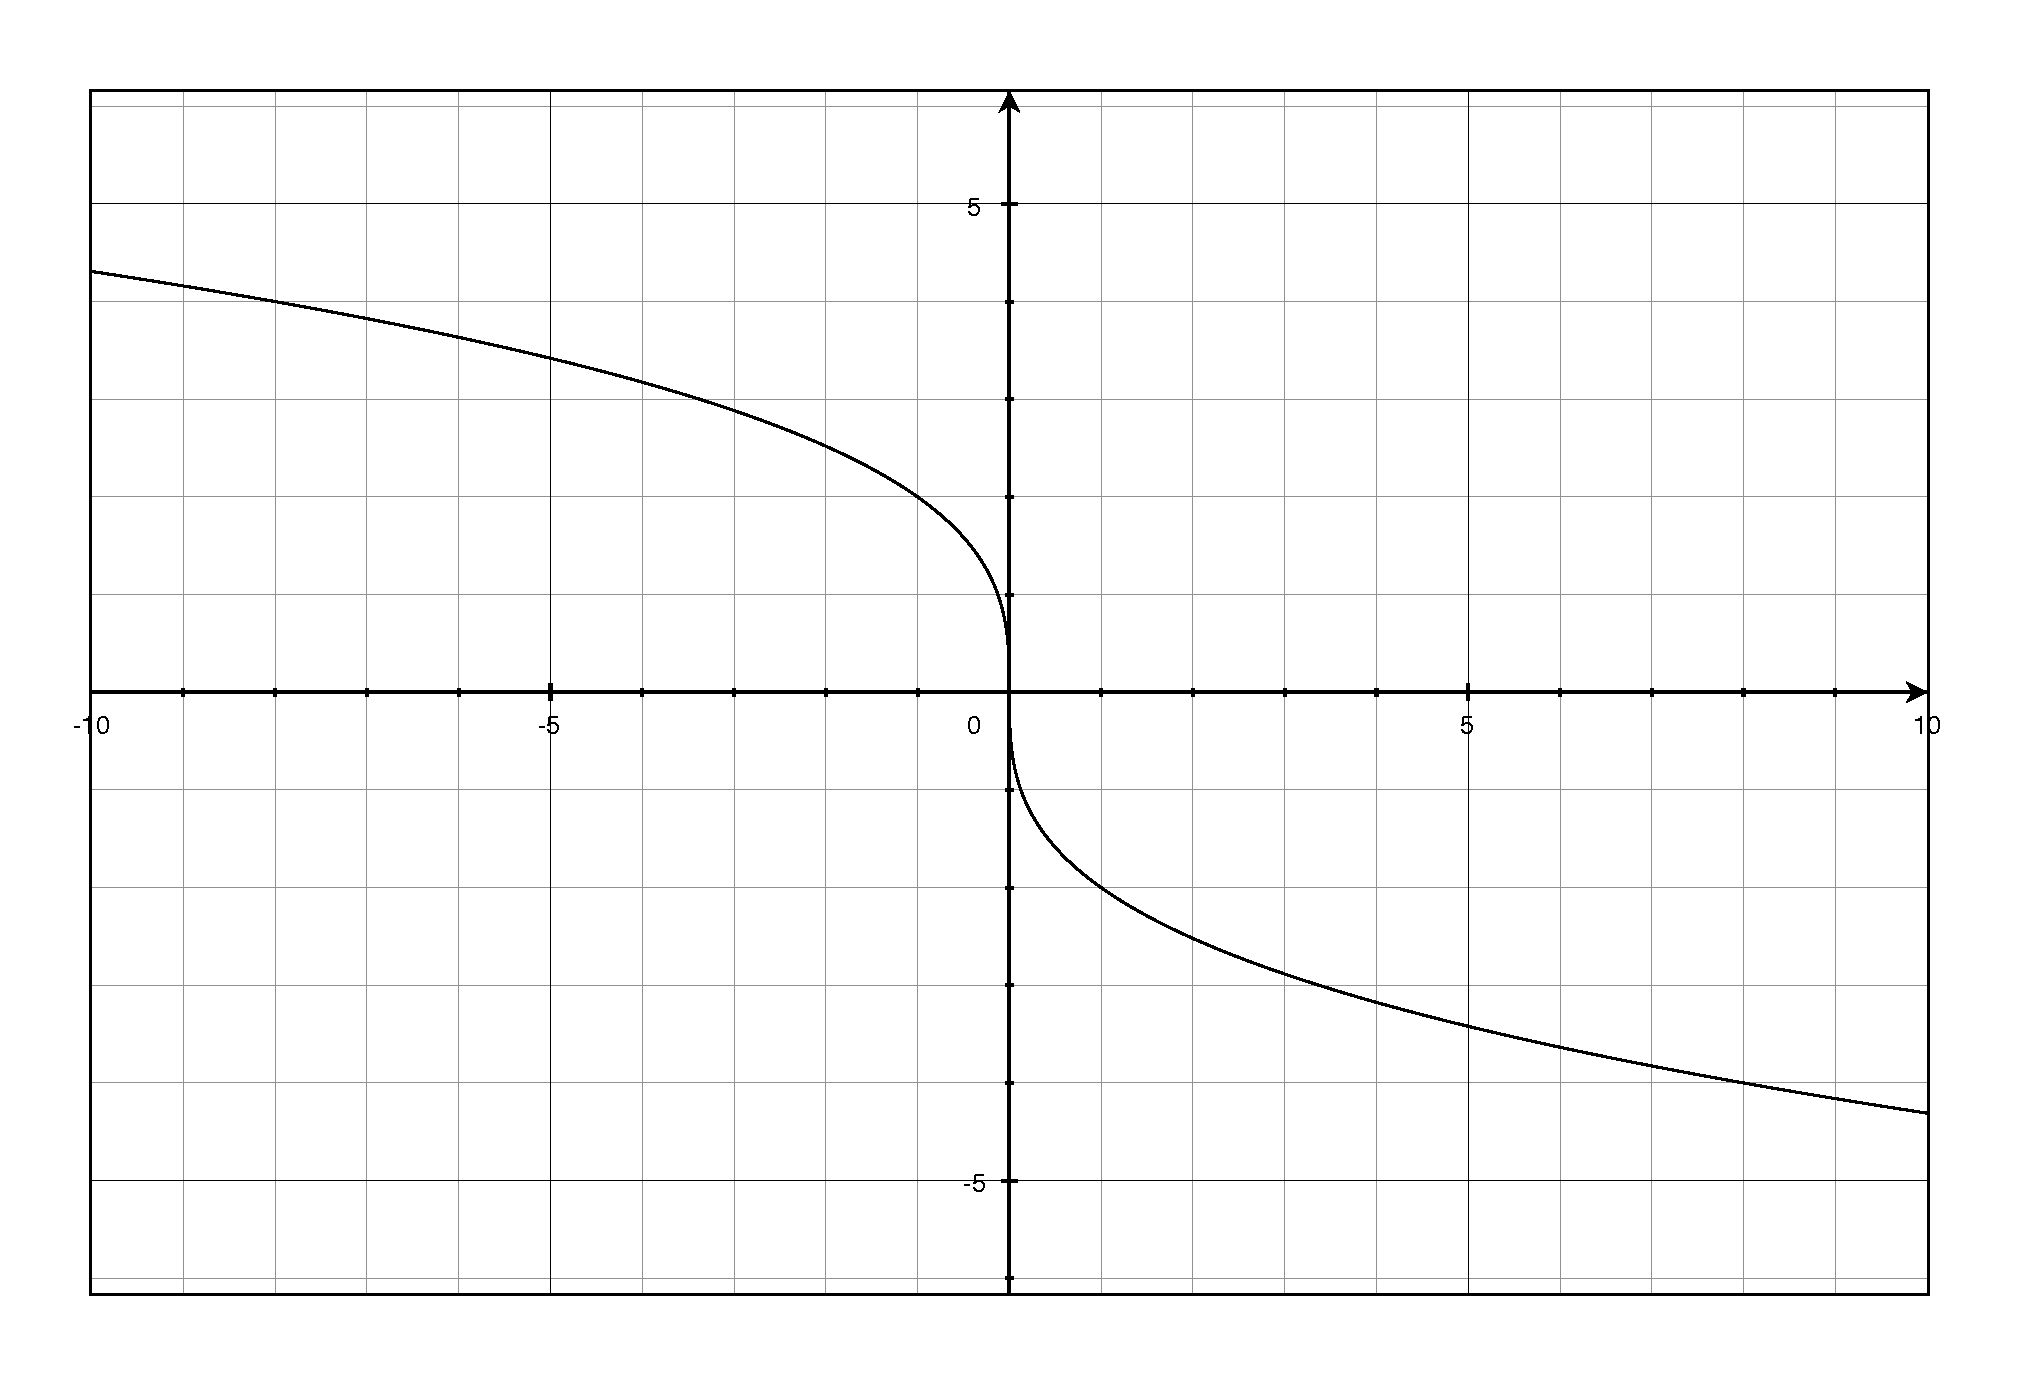
\includegraphics[width=7cm,height=5cm]{1.9-12f.eps}
  \caption*{Problem 12f: $g(x) = -2\sqrt[3]{x}$}
\end{figure}

\item[16]
\begin{align*}
  f(x) &= x^2 - 5x + 6 \\
  &= x^2 - 5x + \frac{25}{4} - \frac{25}{4} + 6 \\
  &= \left(x - \frac{5}{2} \right) ^2 - \frac{25}{4} + \frac{24}{4} \\
  &= \left(x - \frac{5}{2} \right)^2 - \frac{1}{4} \\
\end{align*}

\begin{figure}[H]
  \centering
  \includegraphics[width=7cm,height=5cm]{1.9-16a.eps}
  \caption*{Problem 16: $f(x)$}
\end{figure}

\begin{figure}[H]
  \centering
  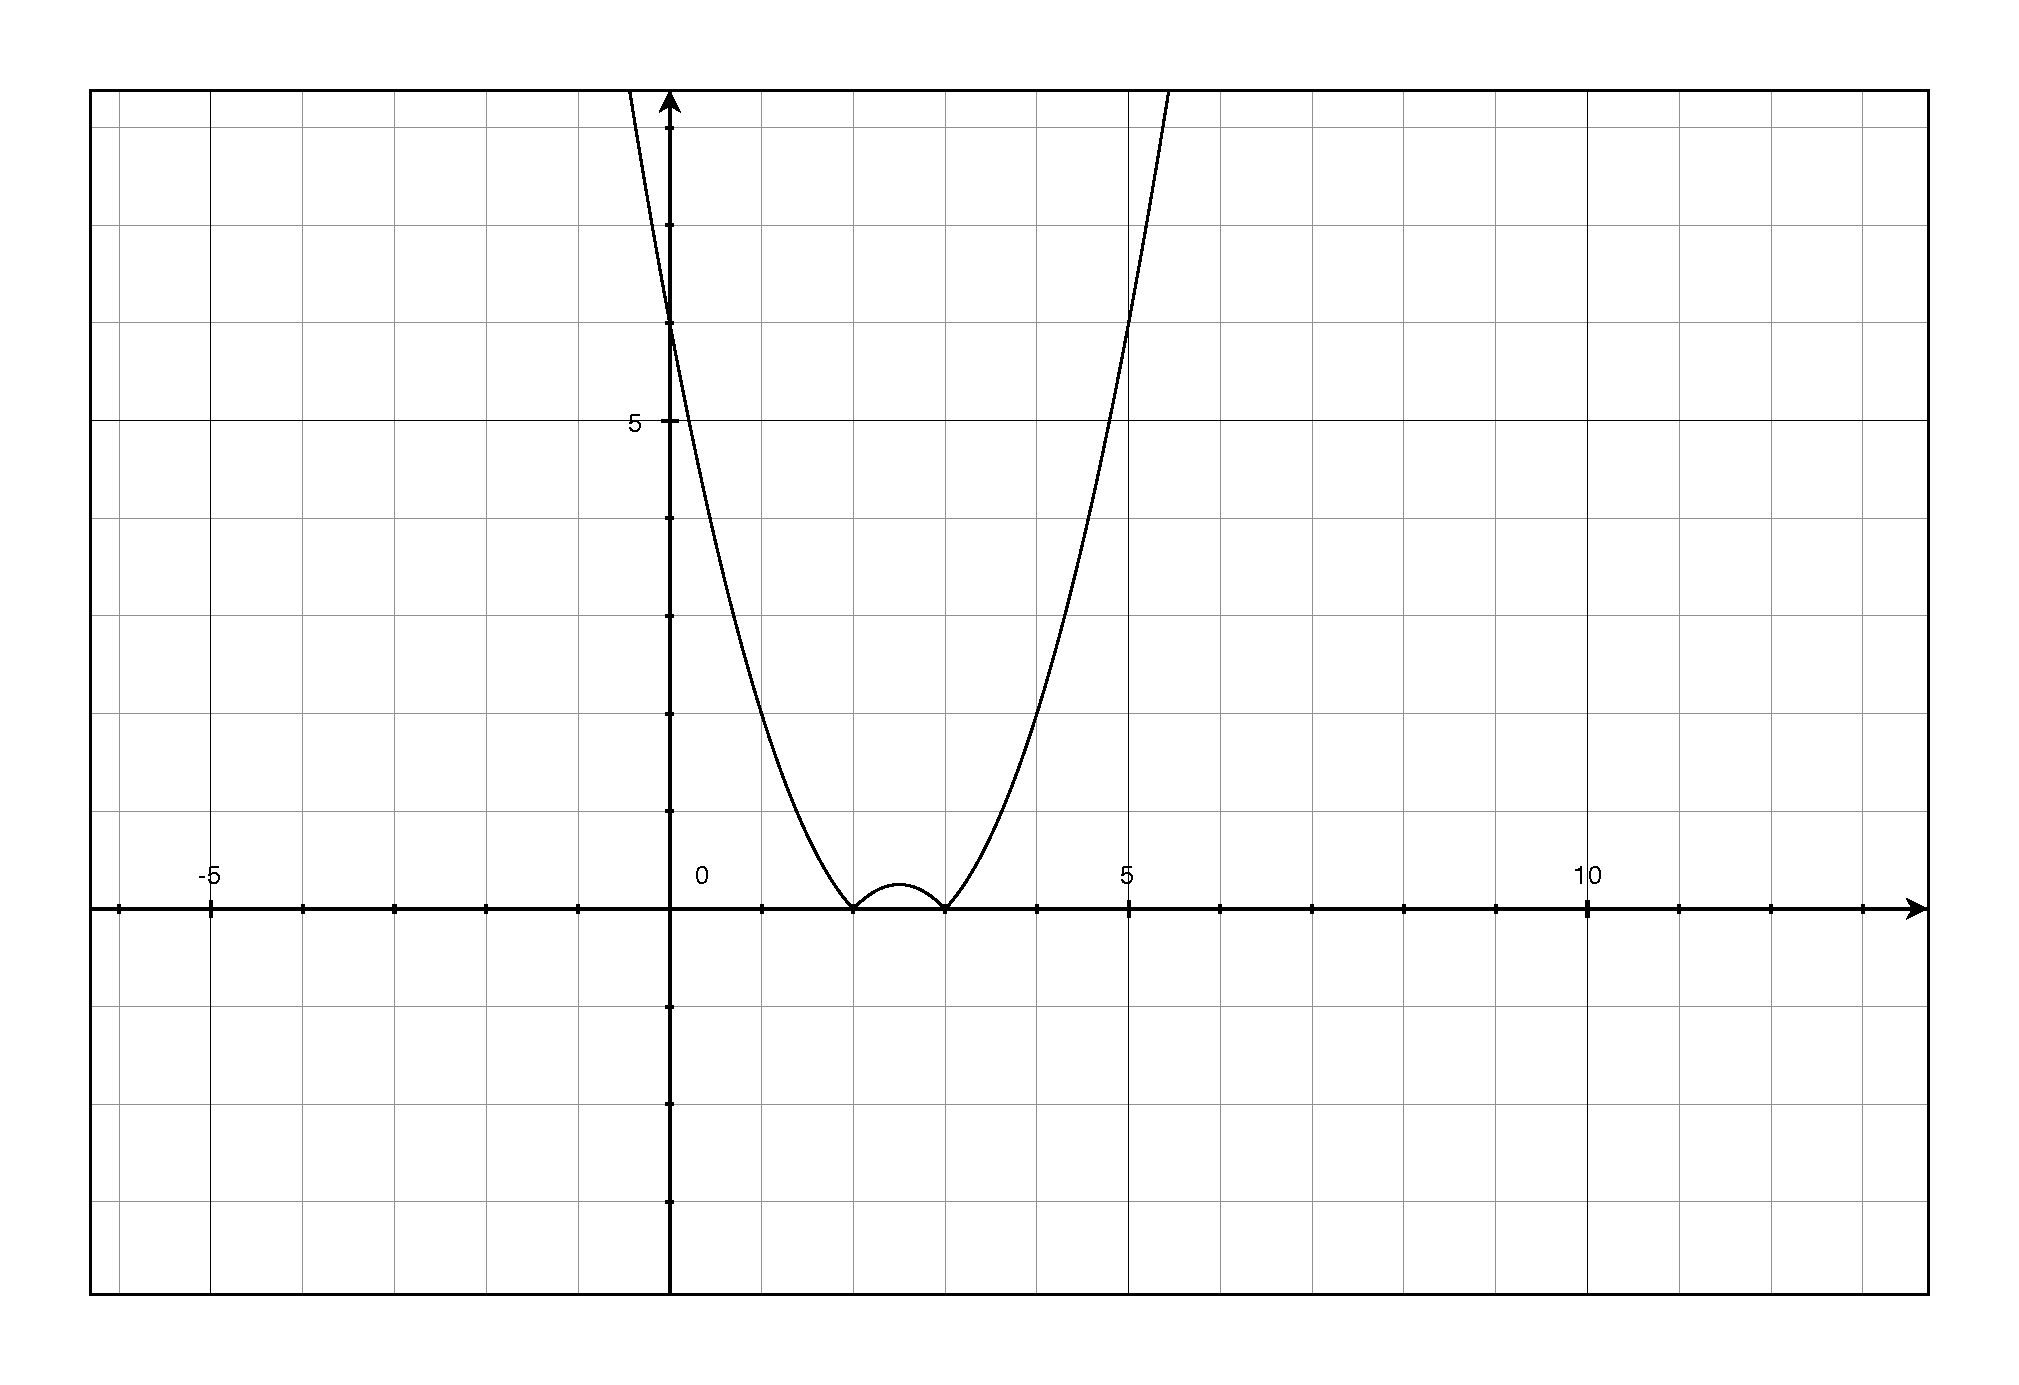
\includegraphics[width=7cm,height=5cm]{1.9-16b.eps}
  \caption*{Problem 16: $|f(x)|$}
\end{figure}

\item[19]
\begin{figure}[H]
  \centering
  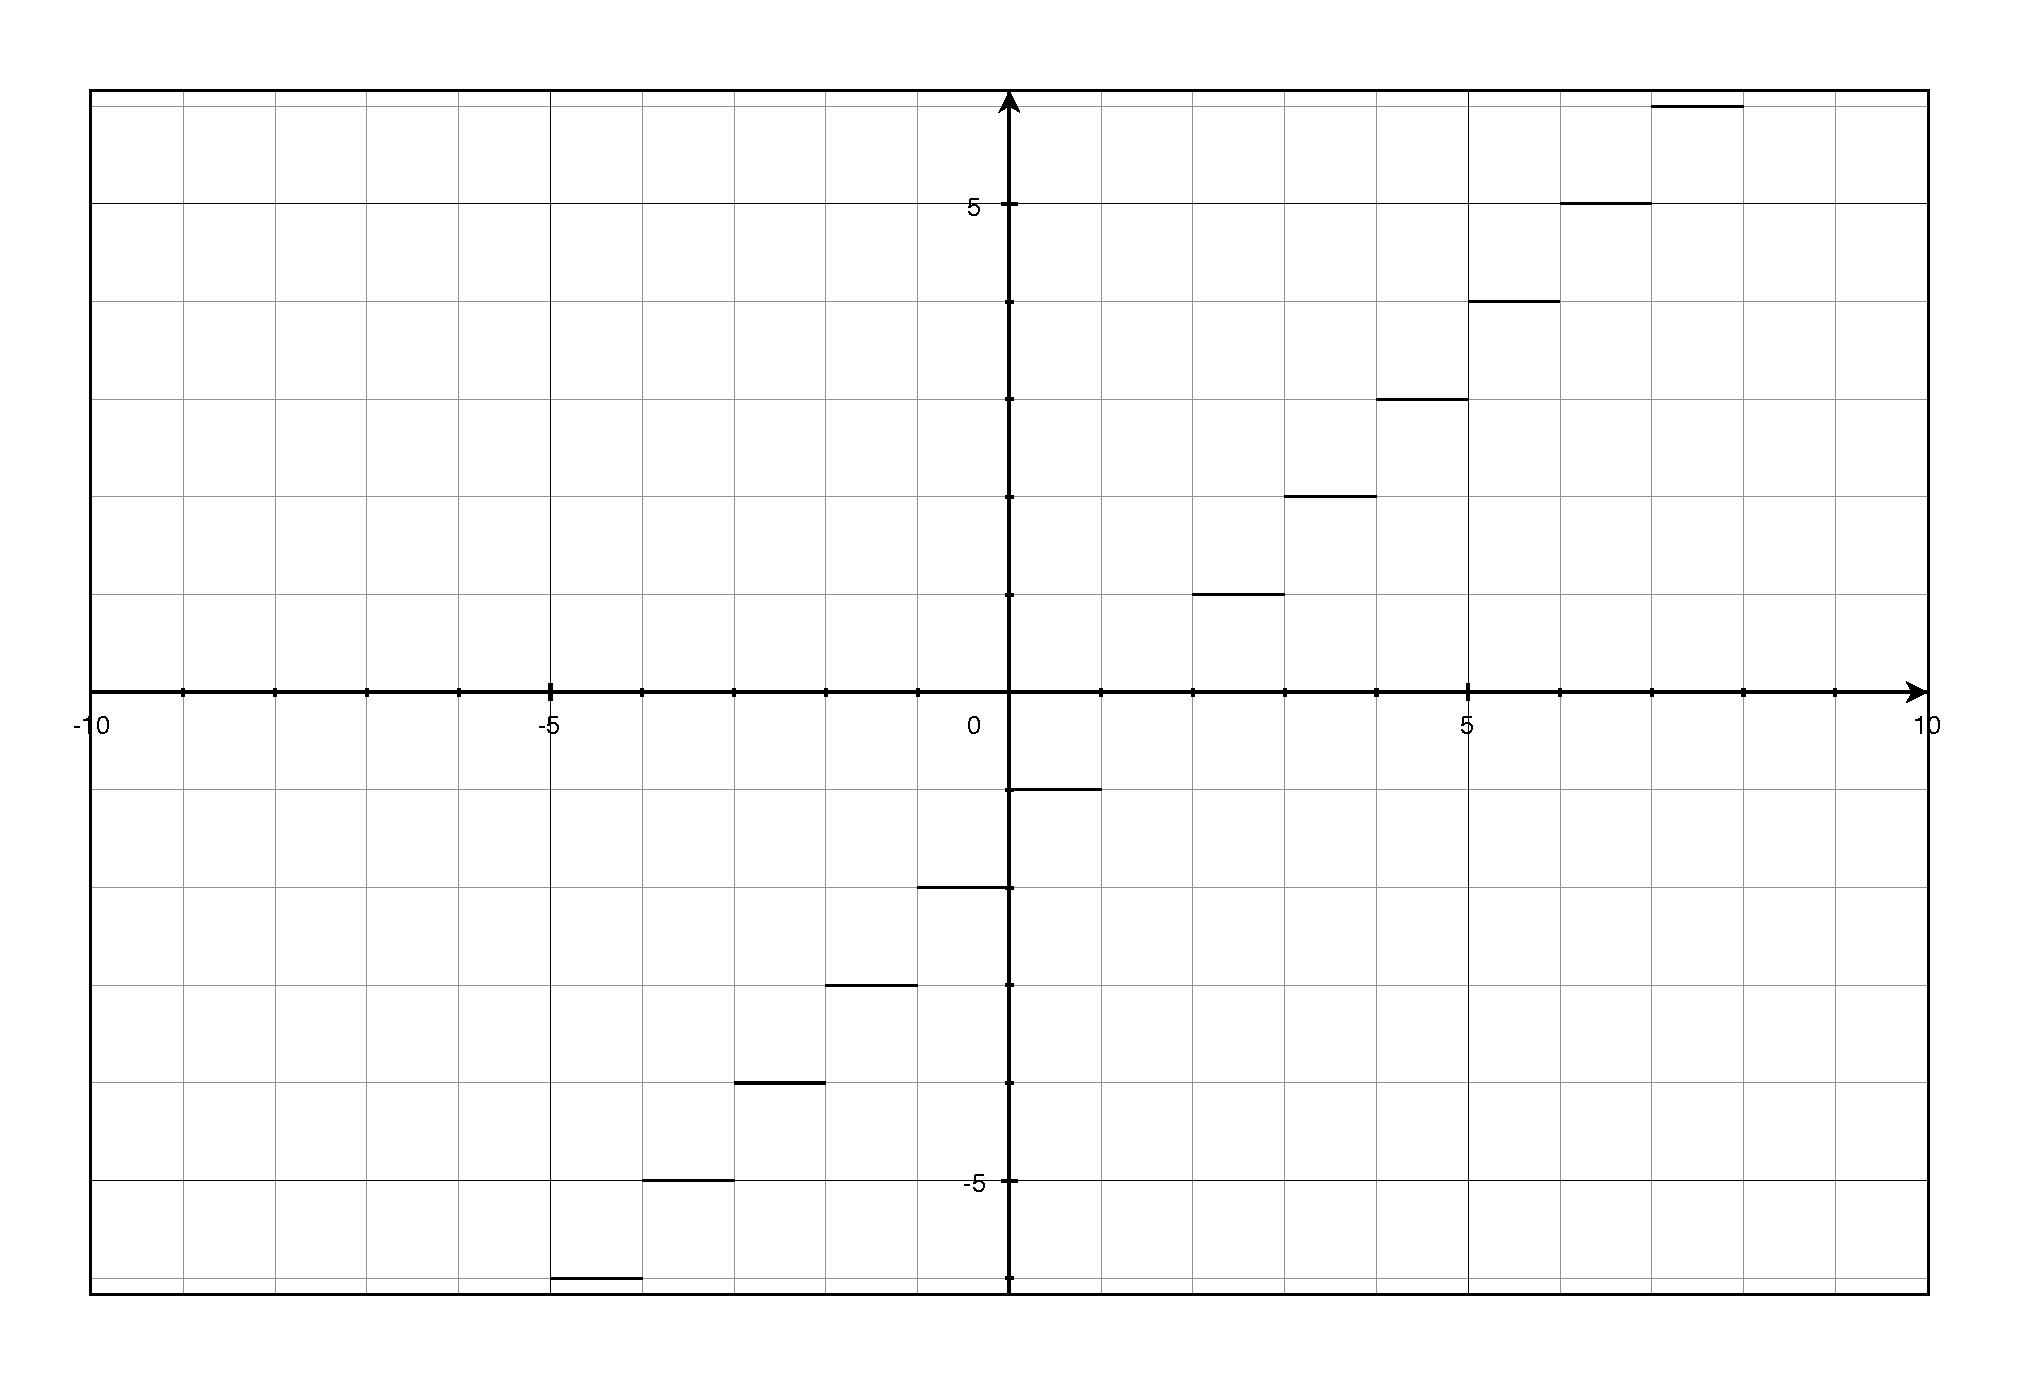
\includegraphics[width=7cm,height=5cm]{1.9-19.eps}
  \caption*{Problem 19}
\end{figure}

\item[23]
From the description, this sounds like an inverted absolute value function, shifted right 1 and down 2:

\[
  f(x) = -|x-1|-2
\]

\begin{figure}[H]
  \centering
  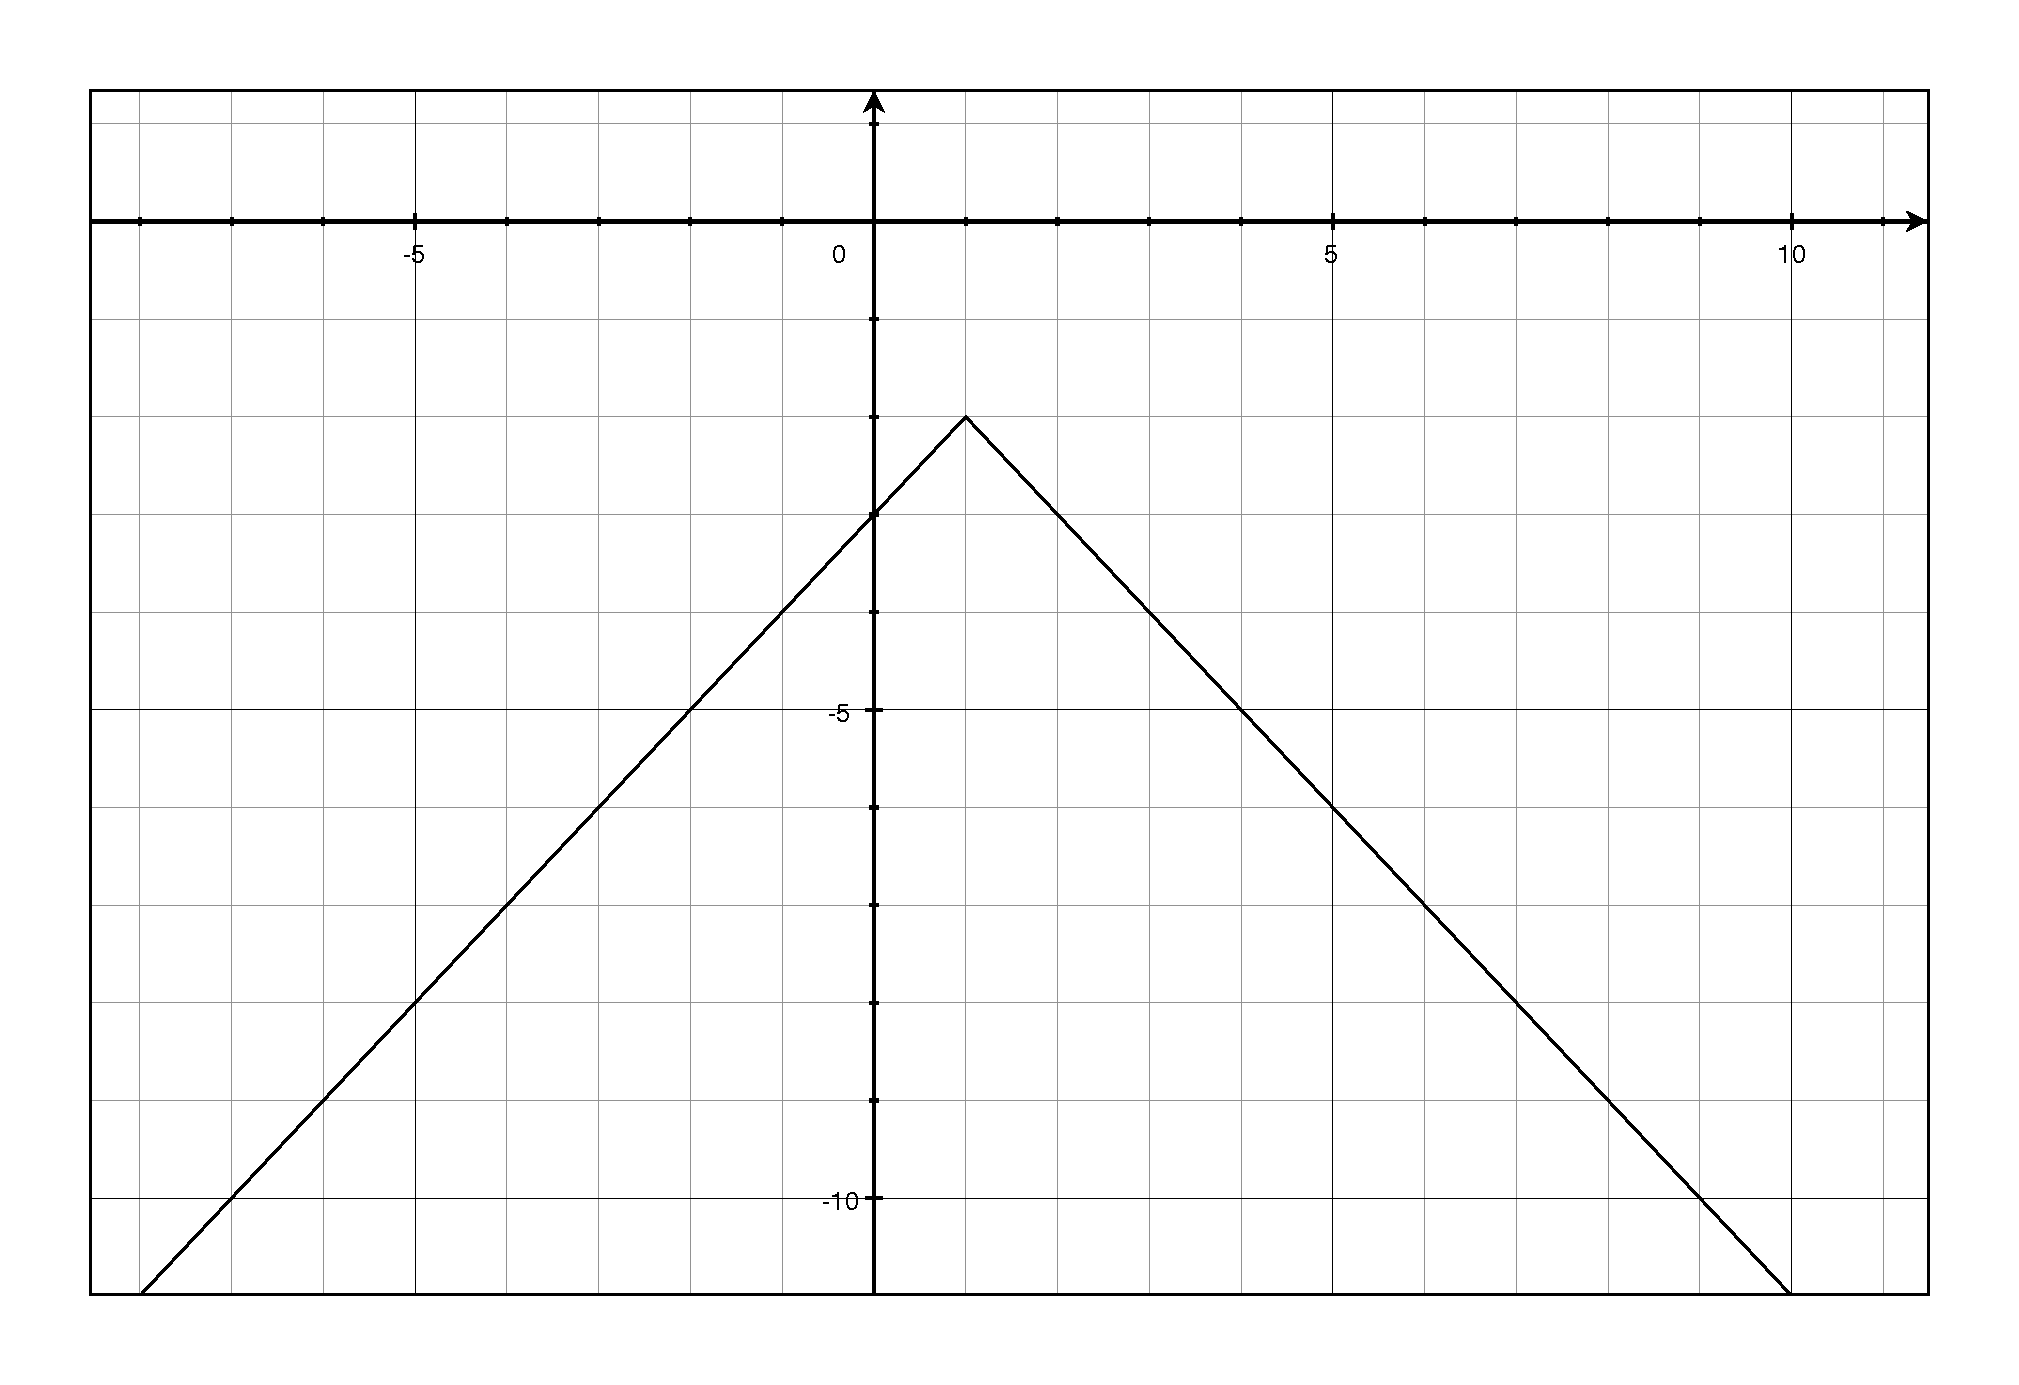
\includegraphics[width=7cm,height=5cm]{1.9-23a.eps}
  \caption*{Problem 23a: $f(x) = -|x-1| - 2$}
\end{figure}

\begin{figure}[H]
  \centering
  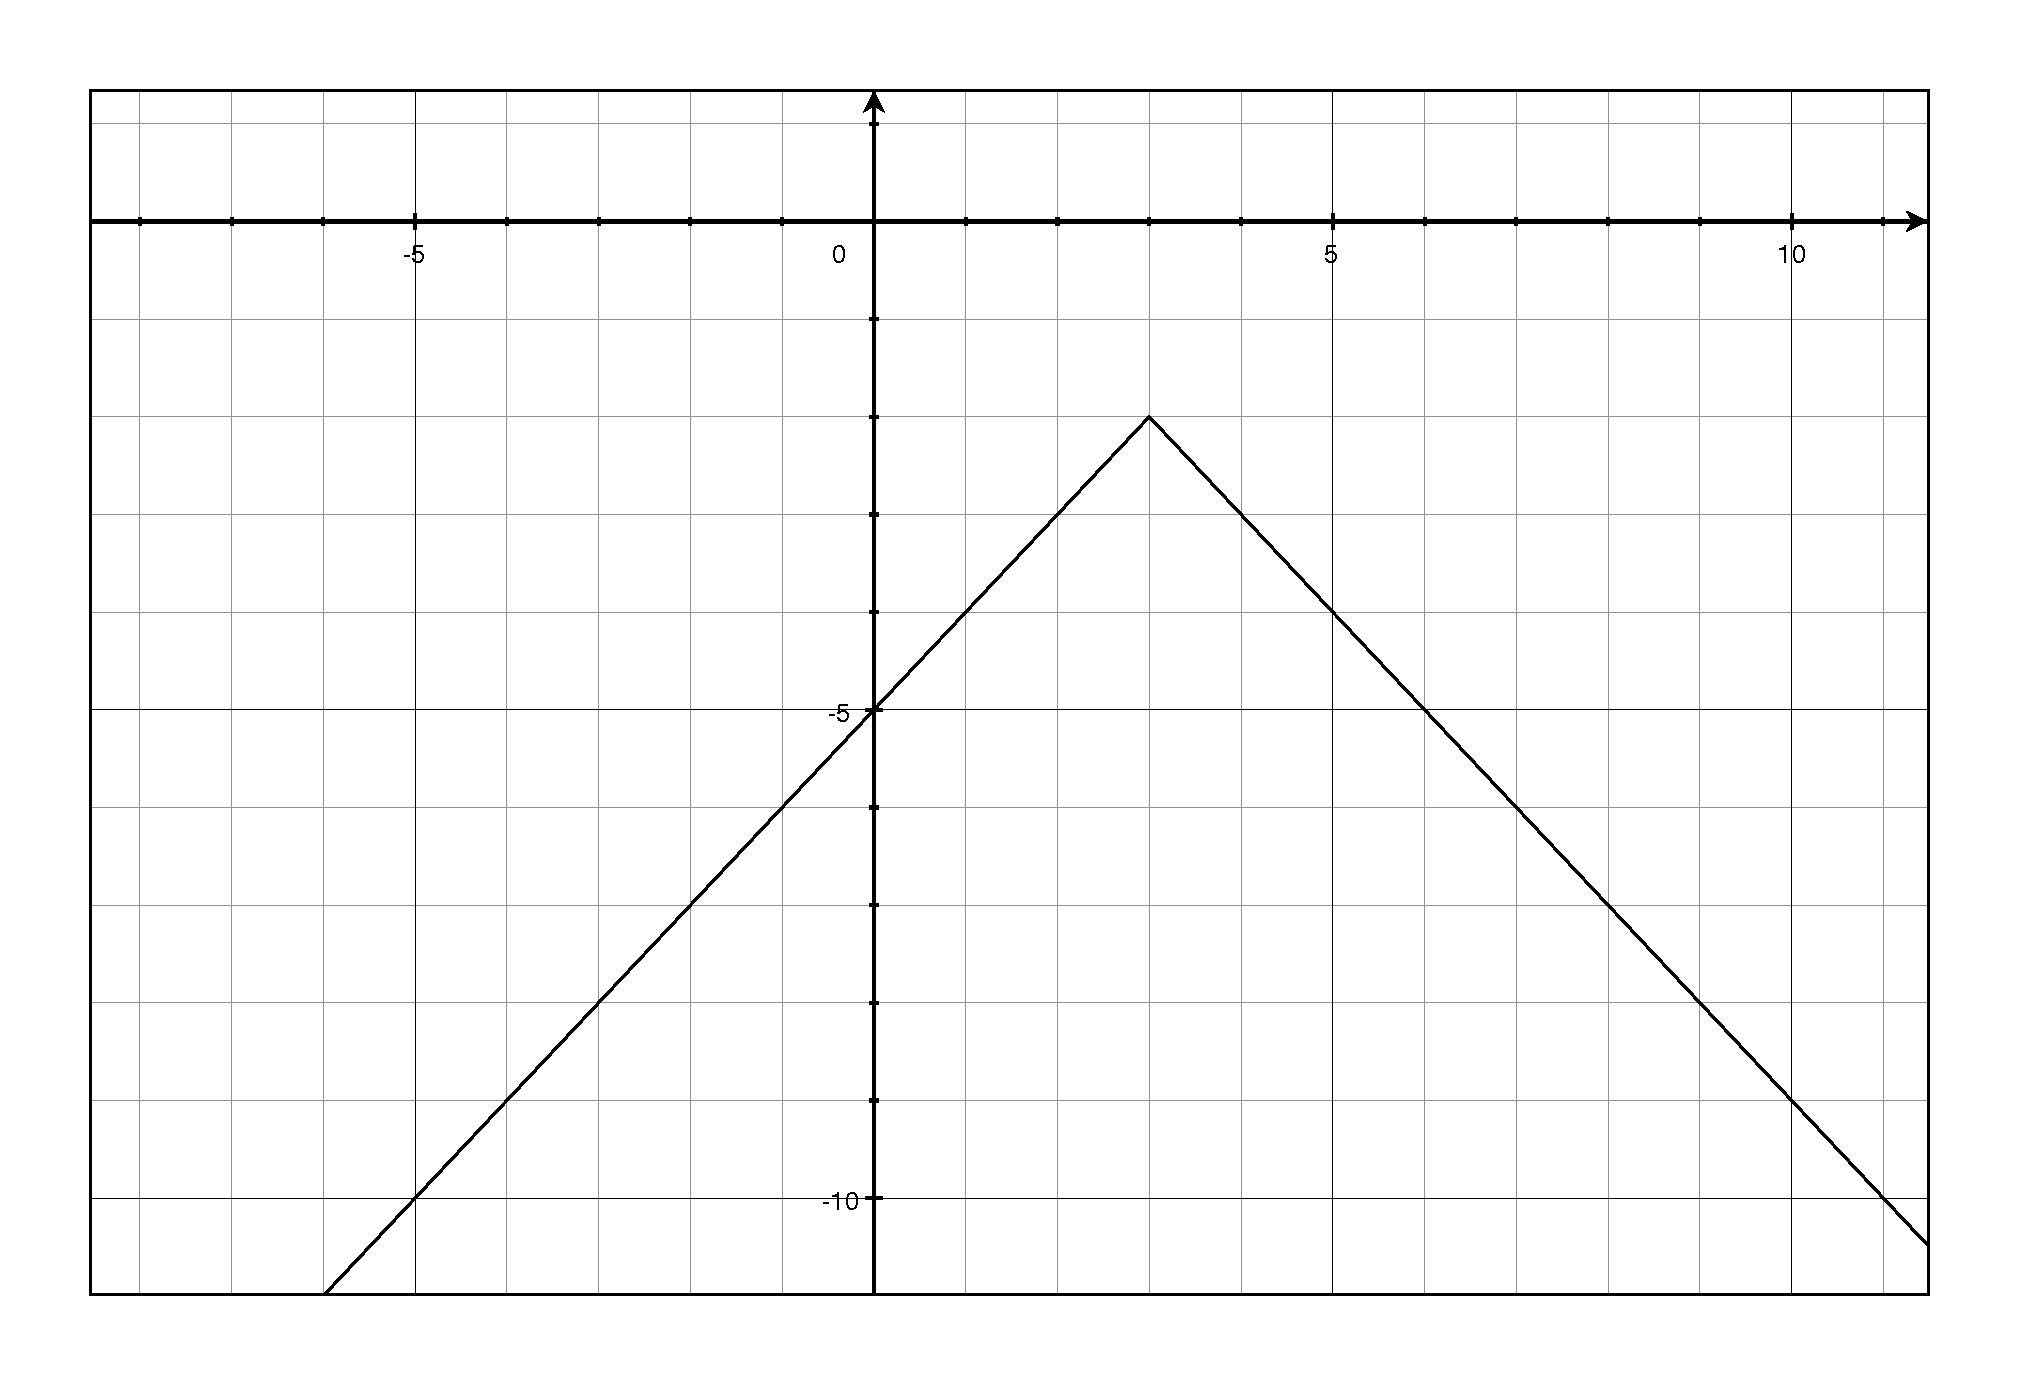
\includegraphics[width=7cm,height=5cm]{1.9-23b.eps}
  \caption*{Problem 23b: $f(x-2) = -|x-3| - 2$}
\end{figure}

\begin{figure}[H]
  \centering
  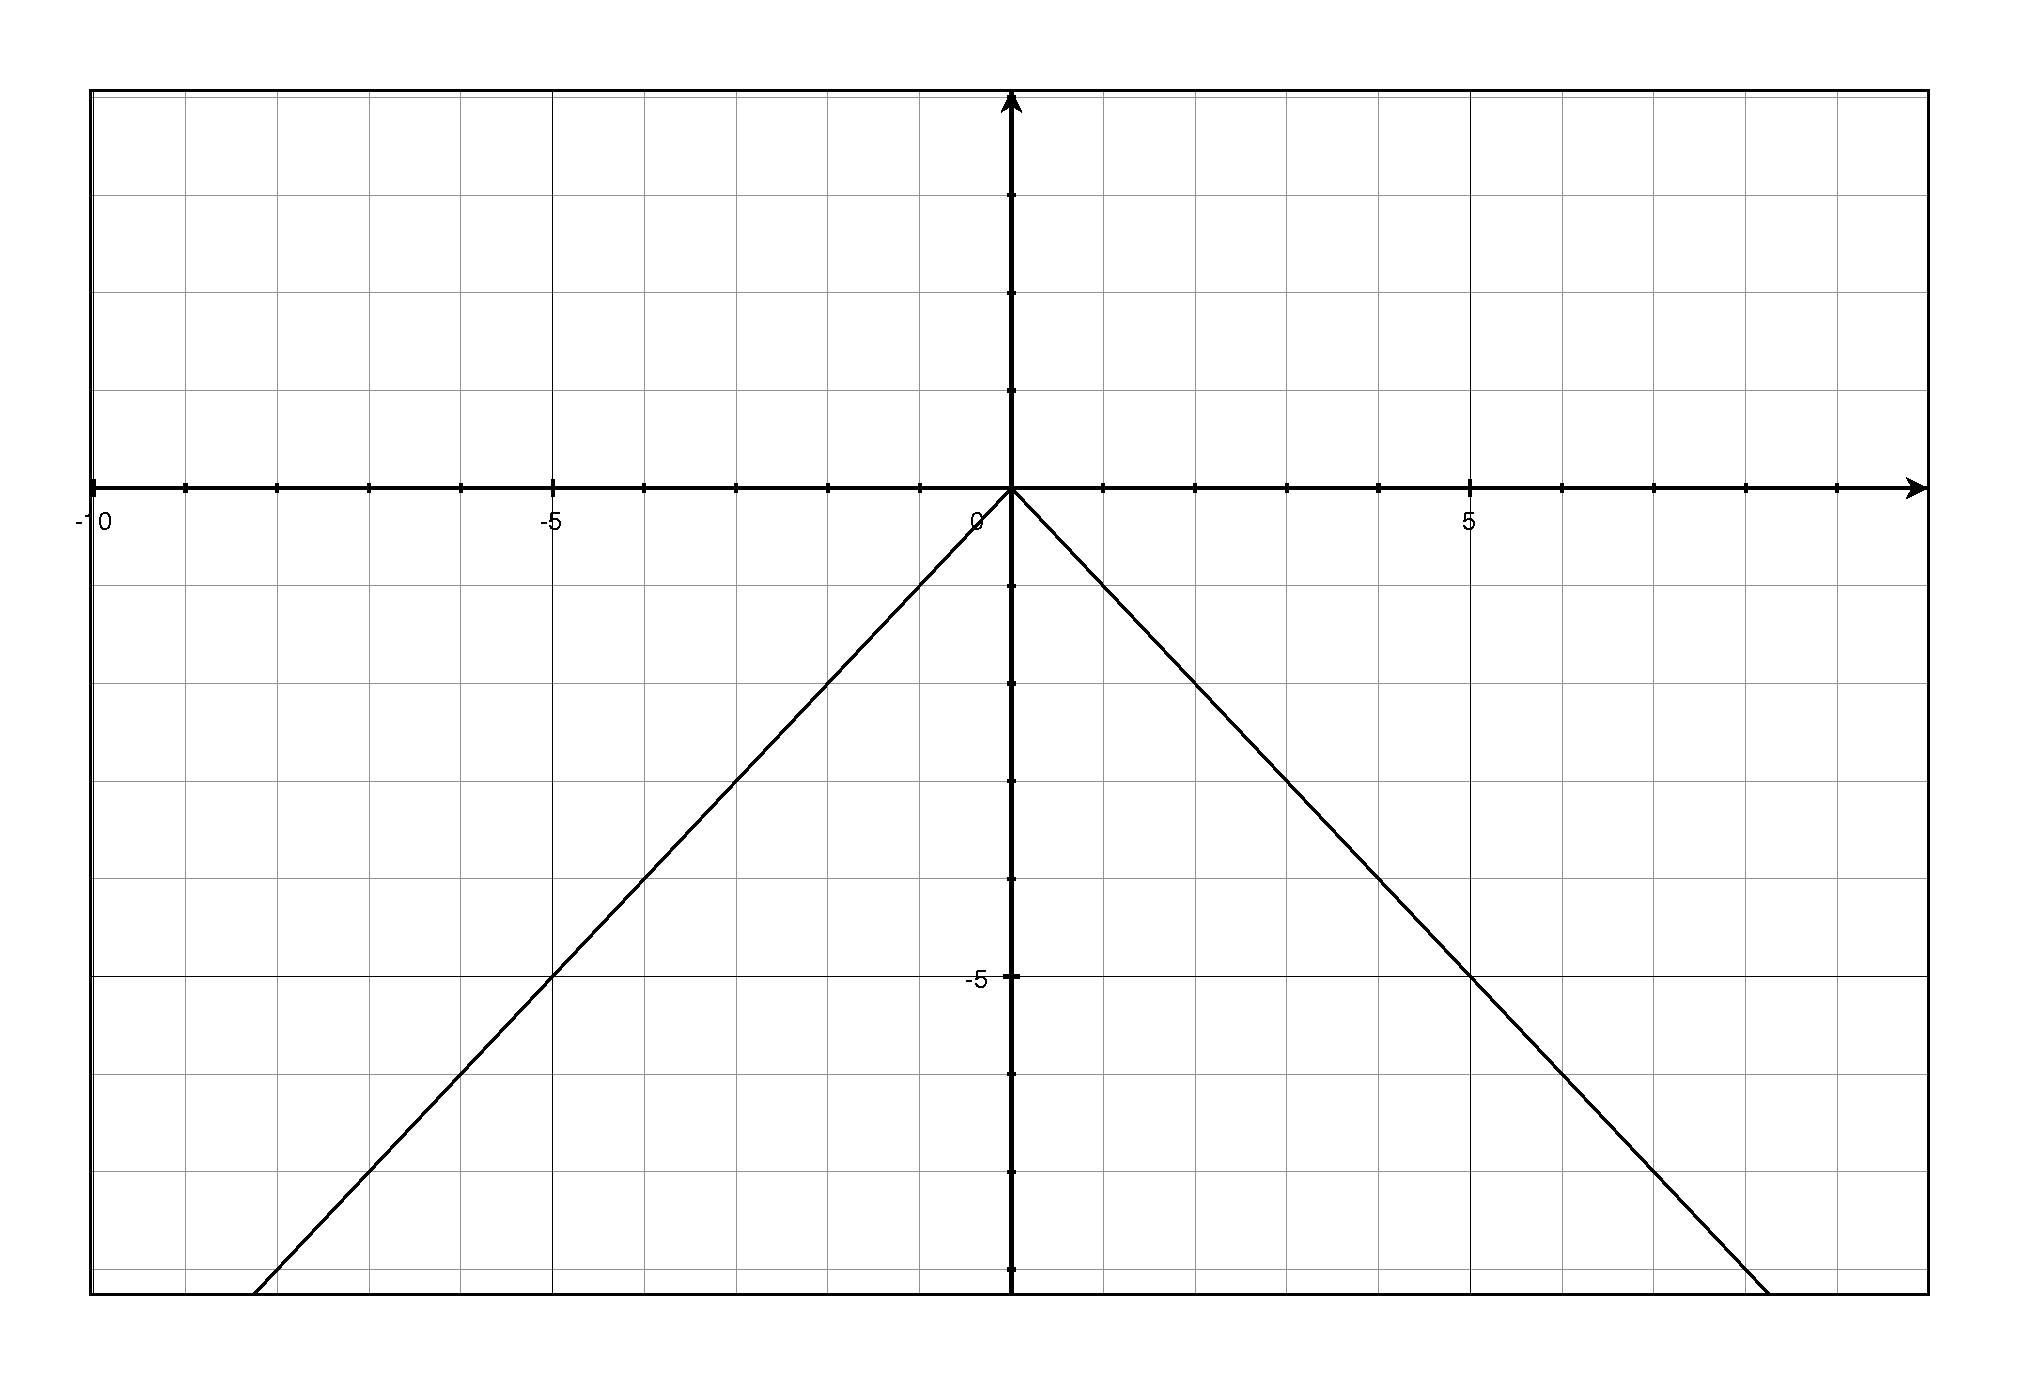
\includegraphics[width=7cm,height=5cm]{1.9-23c.eps}
  \caption*{Problem 23c: $f(x+1) + 2 = |x|$}
\end{figure}

\begin{align*}
  f(3x) &= -|3x-1|-2 \\
        &= -\left| 3(x-\frac{1}{3}) \right| -2 \\
        &= -3 \left| x-\frac{1}{3} \right| -2 \\
\end{align*}

\begin{figure}[H]
  \centering
  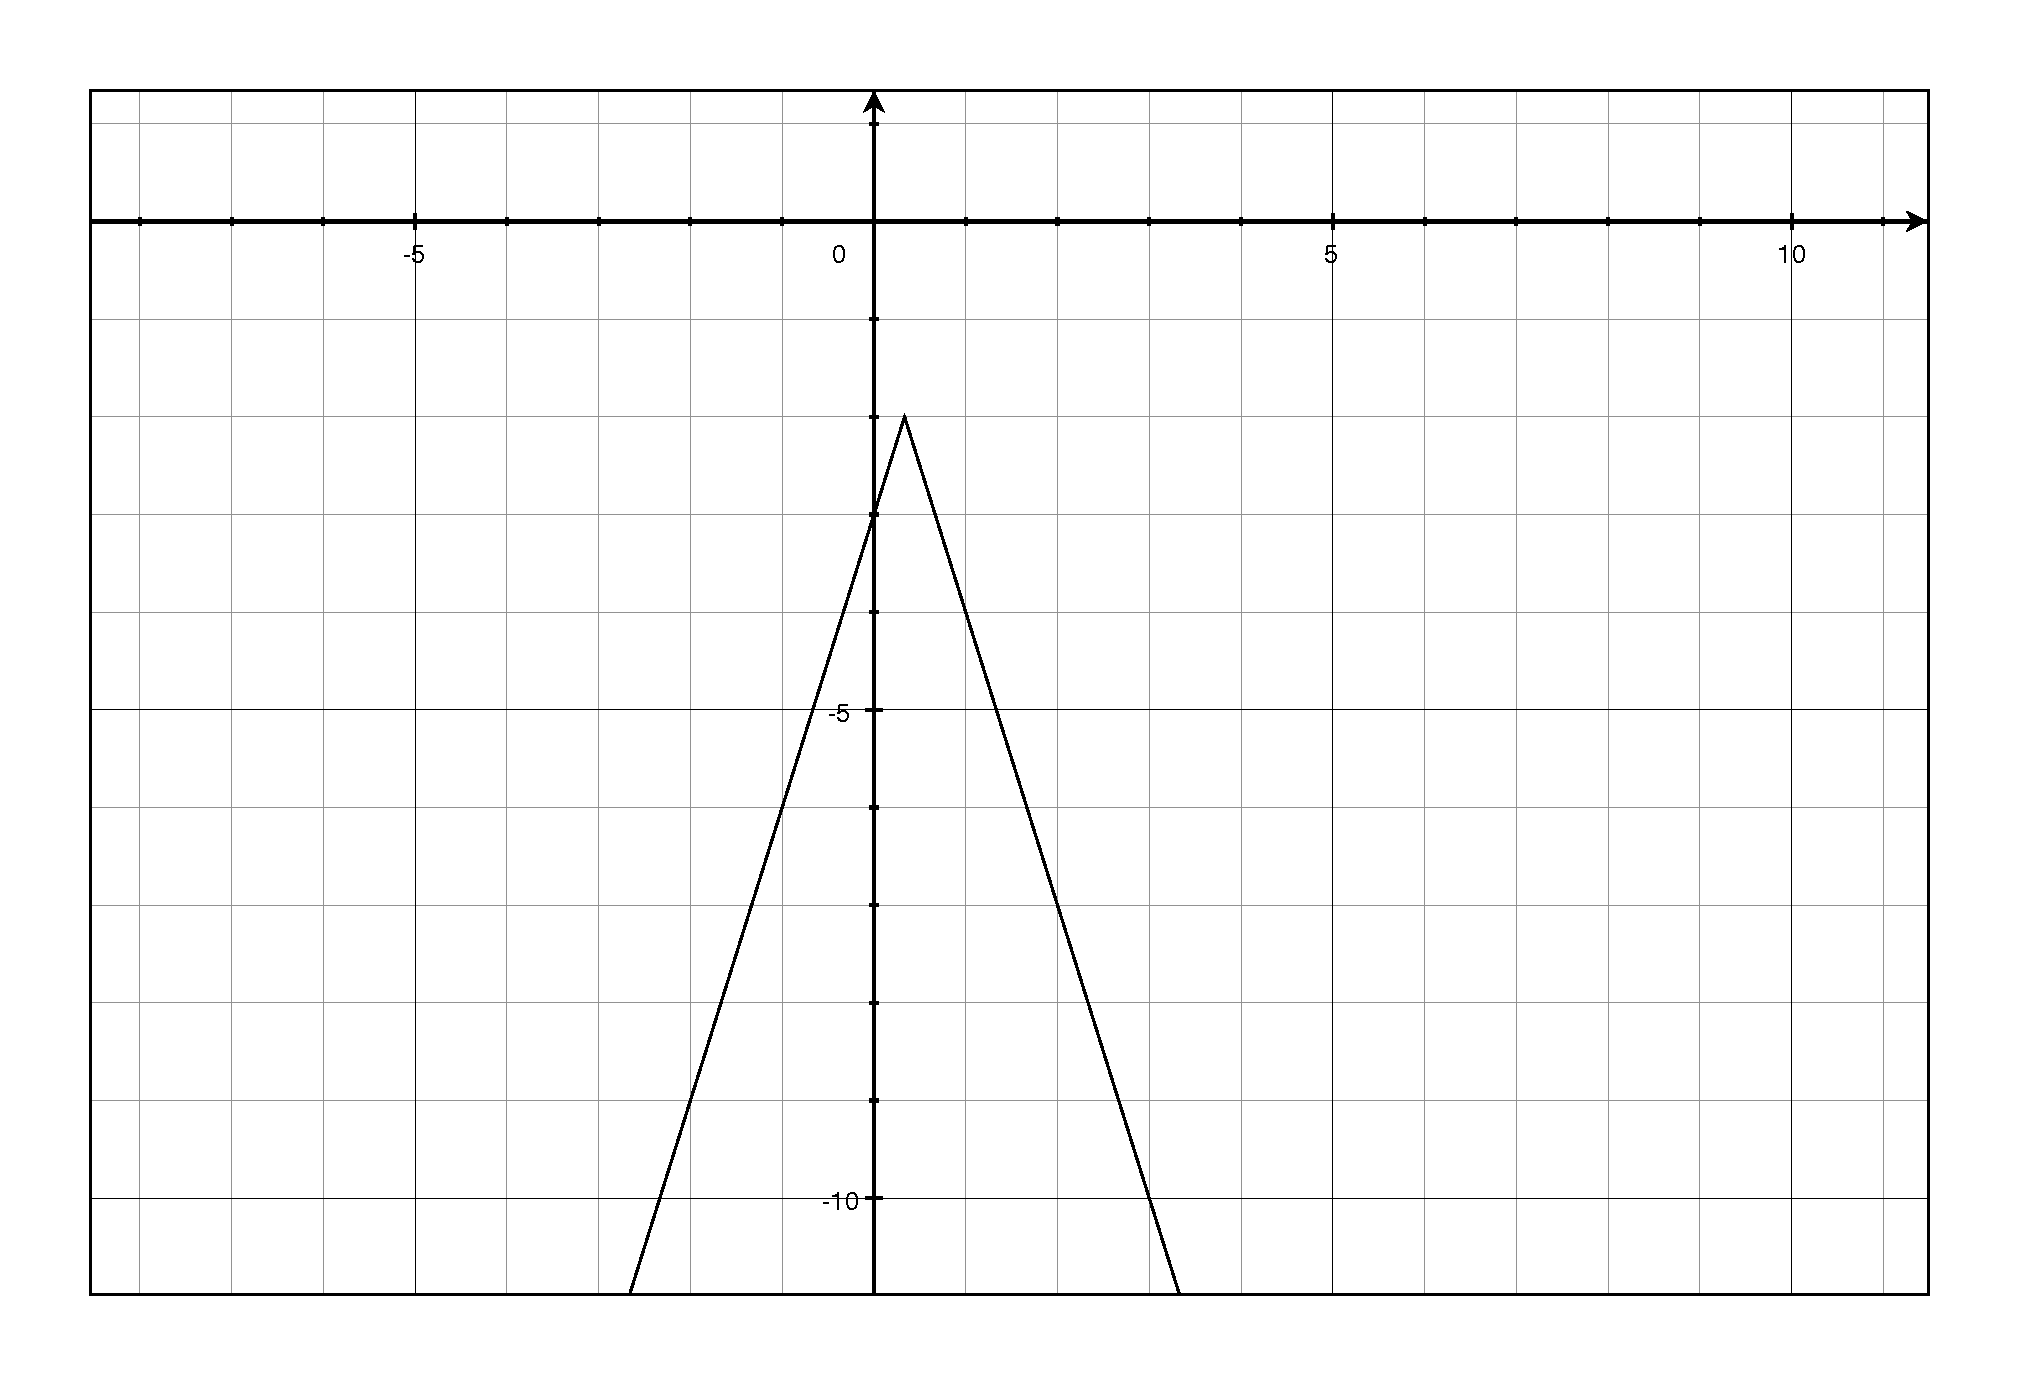
\includegraphics[width=7cm,height=5cm]{1.9-23d.eps}
  \caption*{Problem 23d: $f(3x) = -|3x - 1| - 2$}
\end{figure}

\end{itemize}

\section{Other Problems}

\begin{questions}

\question

Find the vertex and x-intercepts of each function:

\begin{parts}
  \part $f(x) = (x+5)^2 - 6$
\begin{solution}[1cm]
The vertex is: $(-5, 6)$.

To find the x-intercepts, we need to set the $f(x) = 0$ and solve for $x$:
\begin{align*}
  (x+5)^2 - 6 &= 0 \\
  x^2 + 10x + 19 &= 0 \\
\end{align*}

Using the quadratic equation, $x = -5 \pm \sqrt{6}$

\end{solution}

\part $f(x) = x^2 -8x + 16$
\begin{solution}[1cm]

\[
  f(x) = x^2 -8x + 16 = (x-4)^2
\]

So the vertex is at $(4, 0)$ and the only x-intercept is at the vertex.

\end{solution}
\part $f(x) = 2x^2 -x + 1$
\begin{solution}[1cm]

\begin{align*}
  v_x &= \frac{-b}{2a} = \frac{1}{4} \\
  f\left(\frac{1}{4}\right) &= 2\left(\frac{1}{4}\right) - \frac{1}{4} + 1 = \frac{7}{8} \\
\end{align*}

So the vertex is at: $\left( \dfrac{1}{4}, \dfrac{7}{8} \right)$.

There aren't any x-intercepts, since the only solutions of $2x^2 - x +1 = 0$ are imaginary.  There was a typo in this problem, as it was
supposed to have x-intercepts.  The function should have been: $f(x) = 2x^2 - x - 1$ (-1 instead of +1).

\end{solution}

\end{parts}

\question
Use a graphing calculator to graph the function.  Identify the vertex and x-intercepts.  Then check your results
algebraically by completing the square.  

\begin{parts}
  \part $f(x) = -x^2-2x+3$
\begin{solution}[1cm]

vertex:
\begin{align*}
  v_x &= \frac{2}{-2} = -1 \\
  f(-1) &= -(-1)^2 - 2(-1) + 3 = 4
\end{align*}

vertex: $(-1, 4)$

x-intercept:
\begin{align*}
  -x^2-2x+3 &= 0 \\
  x^2+2x-3 &= 0 \\
  (x+3)(x-1) &= 0 \\
\end{align*}

$(-3, 0)$ and $(1, 0)$

\end{solution}

  \part $f(x) = x^2 + 10x + 14$

\begin{solution}[1cm]
vertex:
\begin{align*}
  v_x &= \frac{-10}{2} = -5 \\
  f(-5) &= (-5)^2 + 10(-5) + 14 = -11
\end{align*}

vertex: $(-5, -11)$

x-intercepts:
Using the quadratic formula: $-5 \pm \sqrt{11}$

\end{solution}

\end{parts}

\question
Find the quadratic function that has the indicated vertex and whose graph passes through the given point.
\begin{parts}
  \part Vertex: $(-2, 5)$; Point: $(0, 9)$
\begin{solution}[1cm]
We know the function will look like: 
\[
  f(x) = a(x+2)^2 + 5
\]

We can use the point to find $a$:
\begin{align*}
  9 &= a(0+2)^2 + 5 \\
  a &= 1 \\
\end{align*}

So the function is: $f(x) = (x+2)^2 + 5$


\end{solution}

  \part Vertex: $(4, -1)$; Point: $(2, 3)$
\begin{solution}[1cm]
We know the function will look like: 
\[
  f(x) = a(x-4)^2 - 1
\]

We can use the point to find $a$:
\begin{align*}
  3 &= a(2-4)^2 + 3 \\
  a &= 1 \\
\end{align*}

So the function is: $f(x) = (x-4)^2 - 1$

\end{solution}

\end{parts}

\pagebreak

\section{Extra Credit}

\question
Find the quadratic function whose graph passes through $(6, 4)$, $(1, -1)$ and $(2, -4)$.

\begin{solution}[1cm]

The function will look like: $f(x) = ax^2+bx+c$.  We need to figure out what $a$, $b$, and $c$ are.  We can use the
three points to get three equations:

\begin{align*}
  f(6) &= 4 = a(6)^2 + b(6) + c \\
  f(1) &= -1 = a(1)^2 + b(1) + c \\
  f(2) &= -4 = a(2)^2 + b(2) + c \\
\end{align*}

So we need to solve this system of equations for a, b, and c:
\begin{align*}
  36a + 6b + c &= 4 \\
  a + b + c &= -1 \\
  4a + 2b + c &= -4 \\
\end{align*}

If you do this, you find that $a=1$, $b=-6$, and $c=4$ so the equation is:
\[
  f(x) = x^2 - 6x + 4
\]

\end{solution}

\end{questions}

\ifprintanswers


\fi

\ifprintanswers
\else
\vspace{0.25 cm}

% {\em The more you can increase fear of drugs and crime, welfare mothers, immigrants and aliens, the more you control all
% the people. }

% {\em Under a government which imprisons any unjustly, the true place for a just man is also a prison.}

{\em All voting is a sort of gaming, like checkers or backgammon, with a slight moral tinge to it, a playing with right
  and wrong, with moral questions; and betting naturally accompanies it...A wise man will not
  leave the right to the mercy of chance, nor wish it to prevail through the power of the majority. There is but little
  virtue in the action of masses of men.}

\vspace{.1 cm}
\hspace{1 cm} --Henry David Thoreau

\fi

\end{document}

